% Options for packages loaded elsewhere
\PassOptionsToPackage{unicode}{hyperref}
\PassOptionsToPackage{hyphens}{url}
%
\documentclass[
]{article}
\usepackage{amsmath,amssymb}
\usepackage{iftex}
\ifPDFTeX
  \usepackage[T1]{fontenc}
  \usepackage[utf8]{inputenc}
  \usepackage{textcomp} % provide euro and other symbols
\else % if luatex or xetex
  \usepackage{unicode-math} % this also loads fontspec
  \defaultfontfeatures{Scale=MatchLowercase}
  \defaultfontfeatures[\rmfamily]{Ligatures=TeX,Scale=1}
\fi
\usepackage{lmodern}
\ifPDFTeX\else
  % xetex/luatex font selection
\fi
% Use upquote if available, for straight quotes in verbatim environments
\IfFileExists{upquote.sty}{\usepackage{upquote}}{}
\IfFileExists{microtype.sty}{% use microtype if available
  \usepackage[]{microtype}
  \UseMicrotypeSet[protrusion]{basicmath} % disable protrusion for tt fonts
}{}
\makeatletter
\@ifundefined{KOMAClassName}{% if non-KOMA class
  \IfFileExists{parskip.sty}{%
    \usepackage{parskip}
  }{% else
    \setlength{\parindent}{0pt}
    \setlength{\parskip}{6pt plus 2pt minus 1pt}}
}{% if KOMA class
  \KOMAoptions{parskip=half}}
\makeatother
\usepackage{xcolor}
\usepackage[margin=1in]{geometry}
\usepackage{color}
\usepackage{fancyvrb}
\newcommand{\VerbBar}{|}
\newcommand{\VERB}{\Verb[commandchars=\\\{\}]}
\DefineVerbatimEnvironment{Highlighting}{Verbatim}{commandchars=\\\{\}}
% Add ',fontsize=\small' for more characters per line
\usepackage{framed}
\definecolor{shadecolor}{RGB}{248,248,248}
\newenvironment{Shaded}{\begin{snugshade}}{\end{snugshade}}
\newcommand{\AlertTok}[1]{\textcolor[rgb]{0.94,0.16,0.16}{#1}}
\newcommand{\AnnotationTok}[1]{\textcolor[rgb]{0.56,0.35,0.01}{\textbf{\textit{#1}}}}
\newcommand{\AttributeTok}[1]{\textcolor[rgb]{0.13,0.29,0.53}{#1}}
\newcommand{\BaseNTok}[1]{\textcolor[rgb]{0.00,0.00,0.81}{#1}}
\newcommand{\BuiltInTok}[1]{#1}
\newcommand{\CharTok}[1]{\textcolor[rgb]{0.31,0.60,0.02}{#1}}
\newcommand{\CommentTok}[1]{\textcolor[rgb]{0.56,0.35,0.01}{\textit{#1}}}
\newcommand{\CommentVarTok}[1]{\textcolor[rgb]{0.56,0.35,0.01}{\textbf{\textit{#1}}}}
\newcommand{\ConstantTok}[1]{\textcolor[rgb]{0.56,0.35,0.01}{#1}}
\newcommand{\ControlFlowTok}[1]{\textcolor[rgb]{0.13,0.29,0.53}{\textbf{#1}}}
\newcommand{\DataTypeTok}[1]{\textcolor[rgb]{0.13,0.29,0.53}{#1}}
\newcommand{\DecValTok}[1]{\textcolor[rgb]{0.00,0.00,0.81}{#1}}
\newcommand{\DocumentationTok}[1]{\textcolor[rgb]{0.56,0.35,0.01}{\textbf{\textit{#1}}}}
\newcommand{\ErrorTok}[1]{\textcolor[rgb]{0.64,0.00,0.00}{\textbf{#1}}}
\newcommand{\ExtensionTok}[1]{#1}
\newcommand{\FloatTok}[1]{\textcolor[rgb]{0.00,0.00,0.81}{#1}}
\newcommand{\FunctionTok}[1]{\textcolor[rgb]{0.13,0.29,0.53}{\textbf{#1}}}
\newcommand{\ImportTok}[1]{#1}
\newcommand{\InformationTok}[1]{\textcolor[rgb]{0.56,0.35,0.01}{\textbf{\textit{#1}}}}
\newcommand{\KeywordTok}[1]{\textcolor[rgb]{0.13,0.29,0.53}{\textbf{#1}}}
\newcommand{\NormalTok}[1]{#1}
\newcommand{\OperatorTok}[1]{\textcolor[rgb]{0.81,0.36,0.00}{\textbf{#1}}}
\newcommand{\OtherTok}[1]{\textcolor[rgb]{0.56,0.35,0.01}{#1}}
\newcommand{\PreprocessorTok}[1]{\textcolor[rgb]{0.56,0.35,0.01}{\textit{#1}}}
\newcommand{\RegionMarkerTok}[1]{#1}
\newcommand{\SpecialCharTok}[1]{\textcolor[rgb]{0.81,0.36,0.00}{\textbf{#1}}}
\newcommand{\SpecialStringTok}[1]{\textcolor[rgb]{0.31,0.60,0.02}{#1}}
\newcommand{\StringTok}[1]{\textcolor[rgb]{0.31,0.60,0.02}{#1}}
\newcommand{\VariableTok}[1]{\textcolor[rgb]{0.00,0.00,0.00}{#1}}
\newcommand{\VerbatimStringTok}[1]{\textcolor[rgb]{0.31,0.60,0.02}{#1}}
\newcommand{\WarningTok}[1]{\textcolor[rgb]{0.56,0.35,0.01}{\textbf{\textit{#1}}}}
\usepackage{graphicx}
\makeatletter
\newsavebox\pandoc@box
\newcommand*\pandocbounded[1]{% scales image to fit in text height/width
  \sbox\pandoc@box{#1}%
  \Gscale@div\@tempa{\textheight}{\dimexpr\ht\pandoc@box+\dp\pandoc@box\relax}%
  \Gscale@div\@tempb{\linewidth}{\wd\pandoc@box}%
  \ifdim\@tempb\p@<\@tempa\p@\let\@tempa\@tempb\fi% select the smaller of both
  \ifdim\@tempa\p@<\p@\scalebox{\@tempa}{\usebox\pandoc@box}%
  \else\usebox{\pandoc@box}%
  \fi%
}
% Set default figure placement to htbp
\def\fps@figure{htbp}
\makeatother
\setlength{\emergencystretch}{3em} % prevent overfull lines
\providecommand{\tightlist}{%
  \setlength{\itemsep}{0pt}\setlength{\parskip}{0pt}}
\setcounter{secnumdepth}{-\maxdimen} % remove section numbering
\usepackage{bookmark}
\IfFileExists{xurl.sty}{\usepackage{xurl}}{} % add URL line breaks if available
\urlstyle{same}
\hypersetup{
  pdftitle={Final project},
  pdfauthor={Danny Ahn},
  hidelinks,
  pdfcreator={LaTeX via pandoc}}

\title{Final project}
\author{Danny Ahn}
\date{2025-07-15}

\begin{document}
\maketitle

\section{Introduction}\label{introduction}

The original idea on this project was using Sentence Transformers(SBERT,
for reference view \url{https://sbert.net/}) embedding to classify,
human and AI generated text. However this attempt was unsuccessful
because features that were extracted from SBERT failed to capture any
significant information as shown in t-SNE plot below. Seeing this,
choose to fine tune pretrained LLM RoBERTa.

\begin{figure}
\centering
\pandocbounded{\includegraphics[keepaspectratio]{images/TSNE_plot.png}}
\caption{t-SNE plot of SBERT feature}
\end{figure}

\subsection{Theoretical Background}\label{theoretical-background}

\subsubsection{Perceptrons and Deep
Models}\label{perceptrons-and-deep-models}

\subsubsection{Back propagation and fine
tuning}\label{back-propagation-and-fine-tuning}

\subsubsection{Transformers and attention
mechanism}\label{transformers-and-attention-mechanism}

\subsubsection{RoBERTa and LLM}\label{roberta-and-llm}

In this study, several foundational concepts in natural language
processing and deep learning are used to distinguish between AI- and
human-written texts. \textbf{RoBERTa}, an improved version of BERT, is
employed for its optimized pretraining strategies and enhanced language
understanding. The model architecture is based on the
\textbf{Transformer}, which relies solely on \textbf{attention
mechanisms} to process sequential data efficiently. The attention
mechanism helps the model focus on relevant parts of the input, allowing
better context understanding.

At a lower level, the \textbf{perceptron} serves as the basic unit of
deep neural networks, supporting more complex architectures like
multi-layer networks. \textbf{Large Language Models (LLMs)}, such as
ChatGPT, generate coherent text by predicting word sequences based on
prior data. These models are trained using \textbf{backpropagation}, a
method that calculates gradients using the \textbf{chain rule} to adjust
model parameters.

\textbf{Fine-tuning} is applied to adapt a pre-trained model to a
specific dataset, improving task-specific performance. In this project,
RoBERTa is fine-tuned to classify U.S. Senate press releases as either
human- or AI-generated, utilizing these core principles in a practical
application.

\section{Methods}\label{methods}

Our approach combines sentence-level encoding with a multi-attention
mechanism to classify paragraph-level text. This method is based on our
assumption that GPT will have hard time

\subsubsection{RoBERTector}\label{robertector}

RoBERTector is finetuned RoBerta that specify on AI detection on
sentence level. it's predeictive abilitwes were Accuracy: 0.8648 F1
Score: 0.8644 on validation set.

\subsection{Architecture}\label{architecture}

\begin{figure}
\centering
\pandocbounded{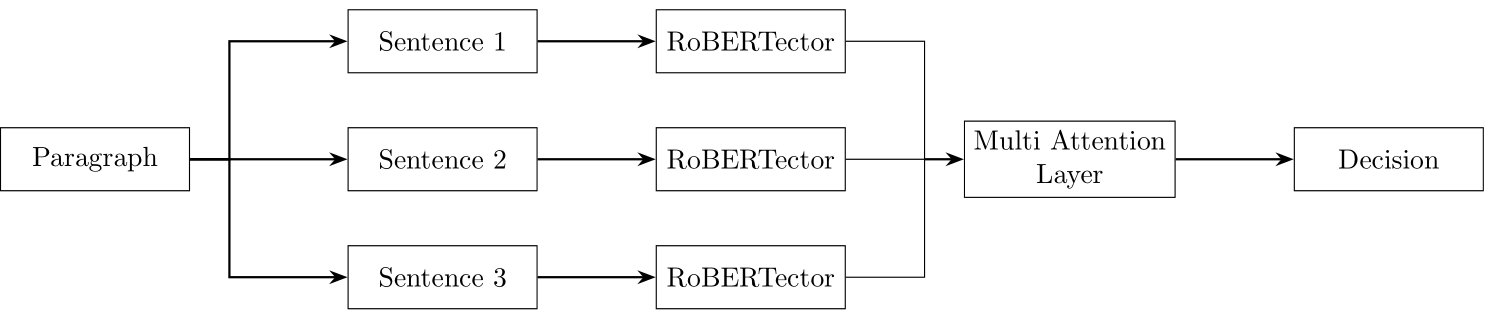
\includegraphics[keepaspectratio]{images/Architecture.png}}
\caption{Architecture}
\end{figure}

Our model begins by \textbf{splitting each paragraph} into at most 16
sentences. We scan for sentence delimiters (\texttt{.}, \texttt{?},
\texttt{!}), trim whitespace, and discard empty fragments. If a
paragraph produces fewer than 16 sentences, we pad the remainder with
dummy tokens; if it exceeds 16, we simply truncate after the 16th. This
approach guarantees every input tensor has a fixed shape
\texttt{(batch\_size\ ×\ 16\ ×\ max\_length)}, which simplifies batching
and avoids dynamic control‐flow overhead.

Next, each of these up to 16 sentence slots is \textbf{encoded
independently} by RoBERTector(a RoBERTa model that was previously
fine‑tuned on sentence‑level AI vs.~human text classification). By
freezing all of RoBERTector's parameters, we preserve its robust ability
to capture subtle stylistic and lexical cues (word choice, phrasing
patterns, function‐word frequencies) without risking over‑fitting on our
comparatively small paragraph dataset. From each sentence's transformer
output we extract the \texttt{CLS} token embedding (a 768‑dimensional
vector), producing a tensor of shape \texttt{(batch\_size,\ 16,\ 768)}.

These 16 sentence embeddings are then fed into a \textbf{multi‑head
self‑attention layer} (four heads, embed\_dim=768). Because the Query,
Key, and Value all derive from the same set of sentence embeddings, the
attention mechanism learns to assign higher weights to the most
informative sentences---thesis statements, topic transitions, or
discourse markers---while down‑weighting less relevant ones. The
attended outputs are mean‑pooled across the sentence axis, yielding a
single 768‑dimensional ``paragraph embedding'' that fuses both
micro‑level sentence cues and macro‑level discourse structure.

Finally, a \textbf{lightweight classification head} (a two‑layer MLP
with ReLU and dropout) maps this paragraph embedding to a single logit.
We apply \texttt{BCEWithLogitsLoss} during training---combining sigmoid
activation and binary cross‑entropy in a numerically stable way---and
use a 0.5 threshold on the sigmoid probability to make the AI vs.~human
decision. We train only the attention and MLP head (leaving RoBERTector
frozen), save model checkpoints after every epoch, and evaluate on an
80/10/10 train/val/test split of our \textasciitilde20\,000‑paragraph
dataset (with test performed just once at the end).

By \textbf{reusing} a specialized sentence encoder, \textbf{learning}
which sentences truly matter via attention, and \textbf{regularizing}
most of the model by freezing, this architecture achieves high accuracy
and generalization while remaining interpretable: attention weights can
be visualized to show exactly which sentences drove each classification.

\section{Training}\label{training}

\subsection{Set up python enviroment}\label{set-up-python-enviroment}

\subsection{Install packages}\label{install-packages}

\subsection{Fine tune RoBERTa}\label{fine-tune-roberta}

\subsubsection{Load data and split paragraphs into
sentences}\label{load-data-and-split-paragraphs-into-sentences}

\begin{Shaded}
\begin{Highlighting}[]
\ImportTok{import}\NormalTok{ pandas }\ImportTok{as}\NormalTok{ pd}
\NormalTok{df}\OperatorTok{=}\NormalTok{pd.read\_csv(}\StringTok{\textquotesingle{}/kaggle/input/ai{-}text/ai\_press\_releases.csv\textquotesingle{}}\NormalTok{)}
\NormalTok{df}\OperatorTok{=}\NormalTok{df.dropna()}
\NormalTok{human}\OperatorTok{=}\NormalTok{df[}\StringTok{\textquotesingle{}non\_chat\_gpt\_press\_release\textquotesingle{}}\NormalTok{]}
\NormalTok{ai}\OperatorTok{=}\NormalTok{df[}\StringTok{\textquotesingle{}chat\_gpt\_generated\_release\textquotesingle{}}\NormalTok{]}
\NormalTok{hu}\OperatorTok{=}\NormalTok{[]}
\NormalTok{a}\OperatorTok{=}\NormalTok{[]}
\ControlFlowTok{for}\NormalTok{ i }\KeywordTok{in}\NormalTok{ human:}
\NormalTok{    l}\OperatorTok{=}\BuiltInTok{list}\NormalTok{(i.split(}\StringTok{\textquotesingle{}. \textquotesingle{}}\NormalTok{))}
\NormalTok{    hu.extend(l)}
\ControlFlowTok{for}\NormalTok{ i }\KeywordTok{in}\NormalTok{ ai:}
\NormalTok{    l}\OperatorTok{=}\BuiltInTok{list}\NormalTok{(i.split(}\StringTok{\textquotesingle{}. \textquotesingle{}}\NormalTok{))}
\NormalTok{    a.extend(l)}

\NormalTok{ap}\OperatorTok{=}\NormalTok{a.copy()}
\NormalTok{a.extend(hu)}
\NormalTok{texts}\OperatorTok{=}\NormalTok{a}
\NormalTok{labels}\OperatorTok{=}\NormalTok{[}\DecValTok{0} \ControlFlowTok{if}\NormalTok{ i}\OperatorTok{\textless{}}\BuiltInTok{len}\NormalTok{(ap) }\ControlFlowTok{else} \DecValTok{1} \ControlFlowTok{for}\NormalTok{ i }\KeywordTok{in} \BuiltInTok{range}\NormalTok{(}\BuiltInTok{len}\NormalTok{(texts))]}
\ImportTok{from}\NormalTok{ sklearn.model\_selection }\ImportTok{import}\NormalTok{ train\_test\_split}

\CommentTok{\#split train, test and validation data. }
\NormalTok{texts\_train\_val, texts\_test, labels\_train\_val, labels\_test }\OperatorTok{=}\NormalTok{ train\_test\_split(}
\NormalTok{    texts,}
\NormalTok{    labels,}
\NormalTok{    test\_size}\OperatorTok{=}\FloatTok{0.2}\NormalTok{,       }\CommentTok{\# 20\% of the entire dataset}
\NormalTok{    random\_state}\OperatorTok{=}\DecValTok{42}\NormalTok{,}
\NormalTok{    stratify}\OperatorTok{=}\NormalTok{labels      }\CommentTok{\# Maintain label distribution}
\NormalTok{)}

\CommentTok{\# 2) Split train\_temp again into train (75\% of temp → 60\% of the total) and val (25\% of temp → 20\% of the total)}
\NormalTok{texts\_train, texts\_val, labels\_train, labels\_val }\OperatorTok{=}\NormalTok{ train\_test\_split(}
\NormalTok{    texts\_train\_val,}
\NormalTok{    labels\_train\_val,}
\NormalTok{    test\_size}\OperatorTok{=}\FloatTok{0.25}\NormalTok{,      }\CommentTok{\#25\% of train\_temp → 0.2 of total}
\NormalTok{    random\_state}\OperatorTok{=}\DecValTok{42}\NormalTok{,}
\NormalTok{    stratify}\OperatorTok{=}\NormalTok{labels\_train\_val}
\NormalTok{)}

\BuiltInTok{print}\NormalTok{(}\SpecialStringTok{f"Train: }\SpecialCharTok{\{}\BuiltInTok{len}\NormalTok{(texts\_train)}\SpecialCharTok{\}}\SpecialStringTok{ samples"}\NormalTok{)}
\BuiltInTok{print}\NormalTok{(}\SpecialStringTok{f"Valid: }\SpecialCharTok{\{}\BuiltInTok{len}\NormalTok{(texts\_val)}\SpecialCharTok{\}}\SpecialStringTok{ samples"}\NormalTok{)}
\BuiltInTok{print}\NormalTok{(}\SpecialStringTok{f"Test : }\SpecialCharTok{\{}\BuiltInTok{len}\NormalTok{(texts\_test)}\SpecialCharTok{\}}\SpecialStringTok{ samples"}\NormalTok{)}
\end{Highlighting}
\end{Shaded}

\subsubsection{Load Roberta and fine
tune}\label{load-roberta-and-fine-tune}

\begin{Shaded}
\begin{Highlighting}[]
\ImportTok{import}\NormalTok{ torch}
\ImportTok{from}\NormalTok{ torch.utils.data }\ImportTok{import}\NormalTok{ DataLoader}
\ImportTok{from}\NormalTok{ transformers }\ImportTok{import}\NormalTok{ AutoTokenizer, AutoModelForSequenceClassification}
\ImportTok{from}\NormalTok{ torch.optim }\ImportTok{import}\NormalTok{ AdamW}
\ImportTok{from}\NormalTok{ datasets }\ImportTok{import}\NormalTok{ Dataset}
\ImportTok{from}\NormalTok{ tqdm.auto }\ImportTok{import}\NormalTok{ tqdm}
\ImportTok{from}\NormalTok{ sklearn.metrics }\ImportTok{import}\NormalTok{ accuracy\_score, f1\_score}

\CommentTok{\# Load pretrained tokenizer}
\NormalTok{tokenizer }\OperatorTok{=}\NormalTok{ AutoTokenizer.from\_pretrained(}\StringTok{"roberta{-}base"}\NormalTok{)}

\CommentTok{\# Function to prepare batch inputs}
\KeywordTok{def}\NormalTok{ collate\_fn(batch):}
\NormalTok{    enc }\OperatorTok{=}\NormalTok{ tokenizer(}
\NormalTok{        [x[}\StringTok{"text"}\NormalTok{] }\ControlFlowTok{for}\NormalTok{ x }\KeywordTok{in}\NormalTok{ batch],  }\CommentTok{\# Extract texts}
\NormalTok{        padding}\OperatorTok{=}\StringTok{"longest"}\NormalTok{,           }\CommentTok{\# Pad to the longest in batch}
\NormalTok{        truncation}\OperatorTok{=}\VariableTok{True}\NormalTok{,             }\CommentTok{\# Truncate if too long}
\NormalTok{        max\_length}\OperatorTok{=}\DecValTok{256}\NormalTok{,              }\CommentTok{\# Limit to 256 tokens}
\NormalTok{        return\_tensors}\OperatorTok{=}\StringTok{"pt"}          \CommentTok{\# Return PyTorch tensors}
\NormalTok{    )}
\NormalTok{    enc[}\StringTok{"labels"}\NormalTok{] }\OperatorTok{=}\NormalTok{ torch.tensor([x[}\StringTok{"label"}\NormalTok{] }\ControlFlowTok{for}\NormalTok{ x }\KeywordTok{in}\NormalTok{ batch], dtype}\OperatorTok{=}\NormalTok{torch.}\BuiltInTok{long}\NormalTok{)}
    \ControlFlowTok{return}\NormalTok{ enc}

\CommentTok{\# Convert to HuggingFace Dataset format}
\NormalTok{train\_ds }\OperatorTok{=}\NormalTok{ Dataset.from\_dict(\{}\StringTok{"text"}\NormalTok{: texts\_train, }\StringTok{"label"}\NormalTok{: labels\_train\})}
\NormalTok{val\_ds   }\OperatorTok{=}\NormalTok{ Dataset.from\_dict(\{}\StringTok{"text"}\NormalTok{: texts\_val,   }\StringTok{"label"}\NormalTok{: labels\_val\})}
\NormalTok{test\_ds  }\OperatorTok{=}\NormalTok{ Dataset.from\_dict(\{}\StringTok{"text"}\NormalTok{: texts\_test,  }\StringTok{"label"}\NormalTok{: labels\_test\})}

\CommentTok{\# Create PyTorch DataLoaders}
\NormalTok{train\_loader }\OperatorTok{=}\NormalTok{ DataLoader(train\_ds, batch\_size}\OperatorTok{=}\DecValTok{16}\NormalTok{, shuffle}\OperatorTok{=}\VariableTok{True}\NormalTok{, collate\_fn}\OperatorTok{=}\NormalTok{collate\_fn)}
\NormalTok{val\_loader   }\OperatorTok{=}\NormalTok{ DataLoader(val\_ds,   batch\_size}\OperatorTok{=}\DecValTok{32}\NormalTok{, shuffle}\OperatorTok{=}\VariableTok{False}\NormalTok{, collate\_fn}\OperatorTok{=}\NormalTok{collate\_fn)}
\NormalTok{test\_loader  }\OperatorTok{=}\NormalTok{ DataLoader(test\_ds,  batch\_size}\OperatorTok{=}\DecValTok{32}\NormalTok{, shuffle}\OperatorTok{=}\VariableTok{False}\NormalTok{, collate\_fn}\OperatorTok{=}\NormalTok{collate\_fn)}

\CommentTok{\# Model and optimizer configuration}
\NormalTok{device }\OperatorTok{=}\NormalTok{ torch.device(}\StringTok{"cuda"} \ControlFlowTok{if}\NormalTok{ torch.cuda.is\_available() }\ControlFlowTok{else} \StringTok{"cpu"}\NormalTok{)  }\CommentTok{\# Use GPU if available}
\NormalTok{model  }\OperatorTok{=}\NormalTok{ AutoModelForSequenceClassification.from\_pretrained(}\StringTok{"roberta{-}base"}\NormalTok{, num\_labels}\OperatorTok{=}\DecValTok{2}\NormalTok{).to(device)  }\CommentTok{\# Binary classification}
\NormalTok{optim  }\OperatorTok{=}\NormalTok{ AdamW(model.parameters(), lr}\OperatorTok{=}\FloatTok{2e{-}5}\NormalTok{)  }\CommentTok{\# Use AdamW optimizer}

\NormalTok{num\_epochs }\OperatorTok{=} \DecValTok{8}  \CommentTok{\# Train for 8 epochs}

\CommentTok{\# Training loop}
\ControlFlowTok{for}\NormalTok{ epoch }\KeywordTok{in} \BuiltInTok{range}\NormalTok{(}\DecValTok{1}\NormalTok{, num\_epochs}\OperatorTok{+}\DecValTok{1}\NormalTok{):}
    \CommentTok{\# 1) Training phase}
\NormalTok{    model.train()}
\NormalTok{    train\_loop }\OperatorTok{=}\NormalTok{ tqdm(train\_loader, desc}\OperatorTok{=}\SpecialStringTok{f"Epoch }\SpecialCharTok{\{}\NormalTok{epoch}\SpecialCharTok{\}}\SpecialStringTok{/}\SpecialCharTok{\{}\NormalTok{num\_epochs}\SpecialCharTok{\}}\SpecialStringTok{ [TRAIN]"}\NormalTok{)  }\CommentTok{\# Show progress}
    \ControlFlowTok{for}\NormalTok{ batch }\KeywordTok{in}\NormalTok{ train\_loop:}
\NormalTok{        batch }\OperatorTok{=}\NormalTok{ \{k: v.to(device) }\ControlFlowTok{for}\NormalTok{ k, v }\KeywordTok{in}\NormalTok{ batch.items()\}  }\CommentTok{\# Move to GPU}
\NormalTok{        outputs }\OperatorTok{=}\NormalTok{ model(}\OperatorTok{**}\NormalTok{batch)  }\CommentTok{\# Forward pass}
\NormalTok{        loss    }\OperatorTok{=}\NormalTok{ outputs.loss}
\NormalTok{        optim.zero\_grad()  }\CommentTok{\# Reset gradients}
\NormalTok{        loss.backward()  }\CommentTok{\# Backpropagation}
\NormalTok{        optim.step()  }\CommentTok{\# Update weights}
\NormalTok{        gpu\_mem }\OperatorTok{=}\NormalTok{ torch.cuda.memory\_allocated(device) }\OperatorTok{//}\NormalTok{ (}\DecValTok{1024}\OperatorTok{**}\DecValTok{2}\NormalTok{)  }\CommentTok{\# Monitor GPU memory}
\NormalTok{        train\_loop.set\_postfix(loss}\OperatorTok{=}\SpecialStringTok{f"}\SpecialCharTok{\{}\NormalTok{loss}\SpecialCharTok{.}\NormalTok{item()}\SpecialCharTok{:.4f\}}\SpecialStringTok{"}\NormalTok{, gpu\_mem}\OperatorTok{=}\SpecialStringTok{f"}\SpecialCharTok{\{}\NormalTok{gpu\_mem}\SpecialCharTok{\}}\SpecialStringTok{MiB"}\NormalTok{)}

    \CommentTok{\# 2) Validation phase}
\NormalTok{    model.}\BuiltInTok{eval}\NormalTok{()}
\NormalTok{    all\_preds, all\_labels }\OperatorTok{=}\NormalTok{ [], []}
\NormalTok{    val\_loop }\OperatorTok{=}\NormalTok{ tqdm(val\_loader, desc}\OperatorTok{=}\SpecialStringTok{f"Epoch }\SpecialCharTok{\{}\NormalTok{epoch}\SpecialCharTok{\}}\SpecialStringTok{/}\SpecialCharTok{\{}\NormalTok{num\_epochs}\SpecialCharTok{\}}\SpecialStringTok{ [VAL]  "}\NormalTok{)}
    \ControlFlowTok{with}\NormalTok{ torch.no\_grad():  }\CommentTok{\# Disable gradient tracking}
        \ControlFlowTok{for}\NormalTok{ batch }\KeywordTok{in}\NormalTok{ val\_loop:}
\NormalTok{            batch }\OperatorTok{=}\NormalTok{ \{k: v.to(device) }\ControlFlowTok{for}\NormalTok{ k, v }\KeywordTok{in}\NormalTok{ batch.items()\}}
\NormalTok{            logits }\OperatorTok{=}\NormalTok{ model(}\OperatorTok{**}\NormalTok{batch).logits}
\NormalTok{            preds  }\OperatorTok{=}\NormalTok{ torch.argmax(logits, dim}\OperatorTok{={-}}\DecValTok{1}\NormalTok{).cpu().tolist()}
\NormalTok{            labels }\OperatorTok{=}\NormalTok{ batch[}\StringTok{"labels"}\NormalTok{].cpu().tolist()}
\NormalTok{            all\_preds }\OperatorTok{+=}\NormalTok{ preds}
\NormalTok{            all\_labels }\OperatorTok{+=}\NormalTok{ labels}
\NormalTok{    val\_acc }\OperatorTok{=}\NormalTok{ accuracy\_score(all\_labels, all\_preds)  }\CommentTok{\# Compute accuracy}
\NormalTok{    val\_f1  }\OperatorTok{=}\NormalTok{ f1\_score(all\_labels, all\_preds, average}\OperatorTok{=}\StringTok{"weighted"}\NormalTok{)  }\CommentTok{\# Compute weighted F1}
    \BuiltInTok{print}\NormalTok{(}\SpecialStringTok{f"→ Validation | Acc: }\SpecialCharTok{\{}\NormalTok{val\_acc}\SpecialCharTok{:.4f\}}\SpecialStringTok{, F1: }\SpecialCharTok{\{}\NormalTok{val\_f1}\SpecialCharTok{:.4f\}}\SpecialStringTok{"}\NormalTok{)}

    \CommentTok{\# 3) Test phase (for monitoring)}
\NormalTok{    all\_preds, all\_labels }\OperatorTok{=}\NormalTok{ [], []}
\NormalTok{    test\_loop }\OperatorTok{=}\NormalTok{ tqdm(test\_loader, desc}\OperatorTok{=}\SpecialStringTok{f"Epoch }\SpecialCharTok{\{}\NormalTok{epoch}\SpecialCharTok{\}}\SpecialStringTok{/}\SpecialCharTok{\{}\NormalTok{num\_epochs}\SpecialCharTok{\}}\SpecialStringTok{ [TEST] "}\NormalTok{)}
    \ControlFlowTok{with}\NormalTok{ torch.no\_grad():}
        \ControlFlowTok{for}\NormalTok{ batch }\KeywordTok{in}\NormalTok{ test\_loop:}
\NormalTok{            batch }\OperatorTok{=}\NormalTok{ \{k: v.to(device) }\ControlFlowTok{for}\NormalTok{ k, v }\KeywordTok{in}\NormalTok{ batch.items()\}}
\NormalTok{            logits }\OperatorTok{=}\NormalTok{ model(}\OperatorTok{**}\NormalTok{batch).logits}
\NormalTok{            preds  }\OperatorTok{=}\NormalTok{ torch.argmax(logits, dim}\OperatorTok{={-}}\DecValTok{1}\NormalTok{).cpu().tolist()}
\NormalTok{            labels }\OperatorTok{=}\NormalTok{ batch[}\StringTok{"labels"}\NormalTok{].cpu().tolist()}
\NormalTok{            all\_preds }\OperatorTok{+=}\NormalTok{ preds}
\NormalTok{            all\_labels }\OperatorTok{+=}\NormalTok{ labels}
\NormalTok{    test\_acc }\OperatorTok{=}\NormalTok{ accuracy\_score(all\_labels, all\_preds)}
\NormalTok{    test\_f1  }\OperatorTok{=}\NormalTok{ f1\_score(all\_labels, all\_preds, average}\OperatorTok{=}\StringTok{"weighted"}\NormalTok{)}
    \BuiltInTok{print}\NormalTok{(}\SpecialStringTok{f"→ Test       | Acc: }\SpecialCharTok{\{}\NormalTok{test\_acc}\SpecialCharTok{:.4f\}}\SpecialStringTok{, F1: }\SpecialCharTok{\{}\NormalTok{test\_f1}\SpecialCharTok{:.4f\}}\SpecialStringTok{"}\NormalTok{)}

    \CommentTok{\# 4) Save model}
\NormalTok{    save\_dir }\OperatorTok{=} \SpecialStringTok{f"/kaggle/working/checkpoint{-}epoch}\SpecialCharTok{\{}\NormalTok{epoch}\SpecialCharTok{\}}\SpecialStringTok{"}  \CommentTok{\# Output directory}
\NormalTok{    model.save\_pretrained(save\_dir)       }\CommentTok{\# Save model weights}
\NormalTok{    tokenizer.save\_pretrained(save\_dir)   }\CommentTok{\# Save tokenizer files}
    \BuiltInTok{print}\NormalTok{(}\SpecialStringTok{f"→ Model \& Tokenizer saved to: }\SpecialCharTok{\{}\NormalTok{save\_dir}\SpecialCharTok{\}}\CharTok{\textbackslash{}n}\SpecialStringTok{"}\NormalTok{)}
\end{Highlighting}
\end{Shaded}

\subsection{Training Multi Attention
Layer}\label{training-multi-attention-layer}

\subsubsection{Load packages}\label{load-packages}

\begin{Shaded}
\begin{Highlighting}[]
\ImportTok{import}\NormalTok{ torch}
\ImportTok{from}\NormalTok{ torch.utils.data }\ImportTok{import}\NormalTok{ DataLoader}
\ImportTok{from}\NormalTok{ transformers }\ImportTok{import}\NormalTok{ AutoTokenizer, AutoModelForSequenceClassification}
\ImportTok{from}\NormalTok{ transformers }\ImportTok{import}\NormalTok{ get\_linear\_schedule\_with\_warmup}
\ImportTok{from}\NormalTok{ torch.optim }\ImportTok{import}\NormalTok{ AdamW}
\ImportTok{from}\NormalTok{ datasets }\ImportTok{import}\NormalTok{ Dataset}
\ImportTok{from}\NormalTok{ tqdm.auto }\ImportTok{import}\NormalTok{ tqdm}
\ImportTok{from}\NormalTok{ sklearn.metrics }\ImportTok{import}\NormalTok{ accuracy\_score, f1\_score}
\ImportTok{import}\NormalTok{ pandas }\ImportTok{as}\NormalTok{ pd}
\ImportTok{from}\NormalTok{ sklearn.model\_selection }\ImportTok{import}\NormalTok{ train\_test\_split}
\ImportTok{import}\NormalTok{ torch.nn }\ImportTok{as}\NormalTok{ nn}
\ImportTok{from}\NormalTok{ torch.utils.data }\ImportTok{import}\NormalTok{ Dataset, DataLoader, random\_split}
\ImportTok{import}\NormalTok{ random}
\ImportTok{import}\NormalTok{ os}
\KeywordTok{def}\NormalTok{ set\_seed(seed}\OperatorTok{=}\DecValTok{42}\NormalTok{):}
\NormalTok{    random.seed(seed)}
\NormalTok{    torch.manual\_seed(seed)}
\NormalTok{    torch.cuda.manual\_seed\_all(seed)}

\NormalTok{set\_seed(}\DecValTok{42}\NormalTok{)}
\end{Highlighting}
\end{Shaded}

\subsubsection{Load data}\label{load-data}

\begin{Shaded}
\begin{Highlighting}[]
\NormalTok{df}\OperatorTok{=}\NormalTok{pd.read\_csv(}\StringTok{\textquotesingle{}/kaggle/input/ai{-}text/ai\_press\_releases.csv\textquotesingle{}}\NormalTok{)}
\NormalTok{df}\OperatorTok{=}\NormalTok{df.dropna()}
\NormalTok{human}\OperatorTok{=}\NormalTok{df[}\StringTok{\textquotesingle{}non\_chat\_gpt\_press\_release\textquotesingle{}}\NormalTok{].to\_list()}
\NormalTok{ai}\OperatorTok{=}\NormalTok{df[}\StringTok{\textquotesingle{}chat\_gpt\_generated\_release\textquotesingle{}}\NormalTok{].to\_list()}
\NormalTok{labels}\OperatorTok{=}\NormalTok{[}\DecValTok{0} \ControlFlowTok{if}\NormalTok{ i}\OperatorTok{\textless{}}\BuiltInTok{len}\NormalTok{(ai) }\ControlFlowTok{else} \DecValTok{1} \ControlFlowTok{for}\NormalTok{ i }\KeywordTok{in} \BuiltInTok{range}\NormalTok{(}\BuiltInTok{len}\NormalTok{(ai)}\OperatorTok{+}\BuiltInTok{len}\NormalTok{(human))]}
\NormalTok{ai.extend(human)}
\NormalTok{texts}\OperatorTok{=}\NormalTok{ai}
\CommentTok{\# 1)split train\_temp(80\%) and test(20\%)}
\NormalTok{texts\_train\_val, texts\_test, labels\_train\_val, labels\_test }\OperatorTok{=}\NormalTok{ train\_test\_split(}
\NormalTok{    texts,}
\NormalTok{    labels,}
\NormalTok{    test\_size}\OperatorTok{=}\FloatTok{0.2}\NormalTok{,       }\CommentTok{\# 20\% of the total}
\NormalTok{    random\_state}\OperatorTok{=}\DecValTok{42}\NormalTok{,}
\NormalTok{    stratify}\OperatorTok{=}\NormalTok{labels      }\CommentTok{\# Maintain label distribution}
\NormalTok{)}

\CommentTok{\# 2) Split train\_temp again into train (75\% of temp → 60\% of the total) and val (25\% of temp → 20\% of the total)}
\NormalTok{texts\_train, texts\_val, labels\_train, labels\_val }\OperatorTok{=}\NormalTok{ train\_test\_split(}
\NormalTok{    texts\_train\_val,}
\NormalTok{    labels\_train\_val,}
\NormalTok{    test\_size}\OperatorTok{=}\FloatTok{0.25}\NormalTok{,      }\CommentTok{\#25\% of train\_temp → 0.2 of total}
\NormalTok{    random\_state}\OperatorTok{=}\DecValTok{42}\NormalTok{,}
\NormalTok{    stratify}\OperatorTok{=}\NormalTok{labels\_train\_val}
\NormalTok{)}

\BuiltInTok{print}\NormalTok{(}\SpecialStringTok{f"Train: }\SpecialCharTok{\{}\BuiltInTok{len}\NormalTok{(texts\_train)}\SpecialCharTok{\}}\SpecialStringTok{ samples"}\NormalTok{)}
\BuiltInTok{print}\NormalTok{(}\SpecialStringTok{f"Valid: }\SpecialCharTok{\{}\BuiltInTok{len}\NormalTok{(texts\_val)}\SpecialCharTok{\}}\SpecialStringTok{ samples"}\NormalTok{)}
\BuiltInTok{print}\NormalTok{(}\SpecialStringTok{f"Test : }\SpecialCharTok{\{}\BuiltInTok{len}\NormalTok{(texts\_test)}\SpecialCharTok{\}}\SpecialStringTok{ samples"}\NormalTok{)}
\end{Highlighting}
\end{Shaded}

\subsubsection{Define helper and Multiattention layer
class}\label{define-helper-and-multiattention-layer-class}

\begin{Shaded}
\begin{Highlighting}[]
\CommentTok{\# 2. Sentence split}
\KeywordTok{def}\NormalTok{ split\_sentences(paragraph: }\BuiltInTok{str}\NormalTok{):}
    \ControlFlowTok{return}\NormalTok{ [s.strip() }\ControlFlowTok{for}\NormalTok{ s }\KeywordTok{in}\NormalTok{ paragraph.split(}\StringTok{\textquotesingle{}. \textquotesingle{}}\NormalTok{) }\ControlFlowTok{if}\NormalTok{ s.strip()]}

\CommentTok{\# 3. Dataset}
\KeywordTok{class}\NormalTok{ ParagraphDataset(Dataset):}
    \KeywordTok{def} \FunctionTok{\_\_init\_\_}\NormalTok{(}\VariableTok{self}\NormalTok{, texts, labels, tokenizer, max\_sents}\OperatorTok{=}\DecValTok{16}\NormalTok{, max\_len}\OperatorTok{=}\DecValTok{128}\NormalTok{):}
        \VariableTok{self}\NormalTok{.texts }\OperatorTok{=}\NormalTok{ texts}
        \VariableTok{self}\NormalTok{.labels }\OperatorTok{=}\NormalTok{ labels}
        \VariableTok{self}\NormalTok{.tokenizer }\OperatorTok{=}\NormalTok{ tokenizer}
        \VariableTok{self}\NormalTok{.max\_sents }\OperatorTok{=}\NormalTok{ max\_sents}
        \VariableTok{self}\NormalTok{.max\_len }\OperatorTok{=}\NormalTok{ max\_len}

    \KeywordTok{def} \FunctionTok{\_\_len\_\_}\NormalTok{(}\VariableTok{self}\NormalTok{):}
        \ControlFlowTok{return} \BuiltInTok{len}\NormalTok{(}\VariableTok{self}\NormalTok{.texts)}

    \KeywordTok{def} \FunctionTok{\_\_getitem\_\_}\NormalTok{(}\VariableTok{self}\NormalTok{, i):}
\NormalTok{        para }\OperatorTok{=} \VariableTok{self}\NormalTok{.texts[i]}
\NormalTok{        label }\OperatorTok{=}\NormalTok{ torch.tensor(}\VariableTok{self}\NormalTok{.labels[i], dtype}\OperatorTok{=}\NormalTok{torch.}\BuiltInTok{float}\NormalTok{)}
\NormalTok{        sents }\OperatorTok{=}\NormalTok{ split\_sentences(para)[:}\VariableTok{self}\NormalTok{.max\_sents]}
\NormalTok{        encs }\OperatorTok{=}\NormalTok{ [}\VariableTok{self}\NormalTok{.tokenizer(s, truncation}\OperatorTok{=}\VariableTok{True}\NormalTok{, padding}\OperatorTok{=}\StringTok{\textquotesingle{}max\_length\textquotesingle{}}\NormalTok{,}
\NormalTok{                               max\_length}\OperatorTok{=}\VariableTok{self}\NormalTok{.max\_len, return\_tensors}\OperatorTok{=}\StringTok{\textquotesingle{}pt\textquotesingle{}}\NormalTok{)}
                \ControlFlowTok{for}\NormalTok{ s }\KeywordTok{in}\NormalTok{ sents]}
        \CommentTok{\# pad sentences}
\NormalTok{        pad\_n }\OperatorTok{=} \VariableTok{self}\NormalTok{.max\_sents }\OperatorTok{{-}} \BuiltInTok{len}\NormalTok{(encs)}
\NormalTok{        input\_ids }\OperatorTok{=}\NormalTok{ torch.stack([e[}\StringTok{\textquotesingle{}input\_ids\textquotesingle{}}\NormalTok{].squeeze(}\DecValTok{0}\NormalTok{) }\ControlFlowTok{for}\NormalTok{ e }\KeywordTok{in}\NormalTok{ encs] }\OperatorTok{+}
\NormalTok{                                [torch.zeros(}\VariableTok{self}\NormalTok{.max\_len, dtype}\OperatorTok{=}\NormalTok{torch.}\BuiltInTok{long}\NormalTok{)]}\OperatorTok{*}\NormalTok{pad\_n)}
\NormalTok{        attn\_mask }\OperatorTok{=}\NormalTok{ torch.stack([e[}\StringTok{\textquotesingle{}attention\_mask\textquotesingle{}}\NormalTok{].squeeze(}\DecValTok{0}\NormalTok{) }\ControlFlowTok{for}\NormalTok{ e }\KeywordTok{in}\NormalTok{ encs] }\OperatorTok{+}
\NormalTok{                                [torch.zeros(}\VariableTok{self}\NormalTok{.max\_len, dtype}\OperatorTok{=}\NormalTok{torch.}\BuiltInTok{long}\NormalTok{)]}\OperatorTok{*}\NormalTok{pad\_n)}
        \ControlFlowTok{return}\NormalTok{ input\_ids, attn\_mask, label}

\CommentTok{\# 4. Model: frozen encoder + attention + classifier}
\ImportTok{import}\NormalTok{ torch}
\ImportTok{import}\NormalTok{ torch.nn }\ImportTok{as}\NormalTok{ nn}
\ImportTok{from}\NormalTok{ transformers }\ImportTok{import}\NormalTok{ AutoTokenizer, AutoModelForSequenceClassification}

\KeywordTok{class}\NormalTok{ HierAttnClassifier(nn.Module):}
    \KeywordTok{def} \FunctionTok{\_\_init\_\_}\NormalTok{(}\VariableTok{self}\NormalTok{,}
\NormalTok{                 base\_model\_name}\OperatorTok{=}\StringTok{"/kaggle/input/robertector/transformers/sentences/1/checkpoint{-}epoch3"}\NormalTok{,}
\NormalTok{                 max\_sents}\OperatorTok{=}\DecValTok{16}\NormalTok{,}
\NormalTok{                 hidden}\OperatorTok{=}\DecValTok{768}\NormalTok{,}
\NormalTok{                 heads}\OperatorTok{=}\DecValTok{4}\NormalTok{):}
        \BuiltInTok{super}\NormalTok{().}\FunctionTok{\_\_init\_\_}\NormalTok{()}
        \CommentTok{\# 1) Load your fine‑tuned SequenceClassification model}
        \VariableTok{self}\NormalTok{.full\_model }\OperatorTok{=}\NormalTok{ AutoModelForSequenceClassification.from\_pretrained(}
\NormalTok{            base\_model\_name, output\_hidden\_states}\OperatorTok{=}\VariableTok{True}\NormalTok{, return\_dict}\OperatorTok{=}\VariableTok{True}
\NormalTok{        )}
        \CommentTok{\# 2) Freeze all its parameters}
        \ControlFlowTok{for}\NormalTok{ p }\KeywordTok{in} \VariableTok{self}\NormalTok{.full\_model.parameters():}
\NormalTok{            p.requires\_grad }\OperatorTok{=} \VariableTok{False}

        \CommentTok{\# 3) Multi‑Head Attention on the CLS embeddings}
        \VariableTok{self}\NormalTok{.attn }\OperatorTok{=}\NormalTok{ nn.MultiheadAttention(embed\_dim}\OperatorTok{=}\NormalTok{hidden,}
\NormalTok{                                          num\_heads}\OperatorTok{=}\NormalTok{heads,}
\NormalTok{                                          batch\_first}\OperatorTok{=}\VariableTok{True}\NormalTok{)}
        \CommentTok{\# 4) Final MLP head after attention}
        \VariableTok{self}\NormalTok{.classifier }\OperatorTok{=}\NormalTok{ nn.Sequential(}
\NormalTok{            nn.Linear(hidden, hidden }\OperatorTok{//} \DecValTok{2}\NormalTok{),}
\NormalTok{            nn.ReLU(),}
\NormalTok{            nn.Dropout(}\FloatTok{0.1}\NormalTok{),}
\NormalTok{            nn.Linear(hidden }\OperatorTok{//} \DecValTok{2}\NormalTok{, }\DecValTok{1}\NormalTok{),}
\NormalTok{        )}

    \KeywordTok{def}\NormalTok{ forward(}\VariableTok{self}\NormalTok{, input\_ids, attention\_mask):}
\NormalTok{        b, s, l }\OperatorTok{=}\NormalTok{ input\_ids.size()}
        \CommentTok{\# flatten to (b*s, l)}
\NormalTok{        flat\_ids   }\OperatorTok{=}\NormalTok{ input\_ids.view(b }\OperatorTok{*}\NormalTok{ s, l)}
\NormalTok{        flat\_mask  }\OperatorTok{=}\NormalTok{ attention\_mask.view(b }\OperatorTok{*}\NormalTok{ s, l)}
        \CommentTok{\# 5) Run through RoBERTector; we asked for hidden\_states}
\NormalTok{        outputs }\OperatorTok{=} \VariableTok{self}\NormalTok{.full\_model(}
\NormalTok{            input\_ids}\OperatorTok{=}\NormalTok{flat\_ids,}
\NormalTok{            attention\_mask}\OperatorTok{=}\NormalTok{flat\_mask,}
\NormalTok{        )}
        \CommentTok{\# 6) Grab the last hidden layer states: outputs.hidden\_states is a tuple}
        \CommentTok{\#    where hidden\_states[{-}1] is (batch, seq\_len, hidden)}
\NormalTok{        last\_hid }\OperatorTok{=}\NormalTok{ outputs.hidden\_states[}\OperatorTok{{-}}\DecValTok{1}\NormalTok{]        }
        \CommentTok{\# CLS is token 0}
\NormalTok{        cls\_embs }\OperatorTok{=}\NormalTok{ last\_hid[:, }\DecValTok{0}\NormalTok{, :].view(b, s, }\OperatorTok{{-}}\DecValTok{1}\NormalTok{)  }\CommentTok{\# (b, s, hidden)}

        \CommentTok{\# 7) Self‑attention over the s sentence embeddings}
\NormalTok{        attn\_out, \_ }\OperatorTok{=} \VariableTok{self}\NormalTok{.attn(cls\_embs, cls\_embs, cls\_embs)  }\CommentTok{\# (b, s, hidden)}

        \CommentTok{\# 8) Pool and classify}
\NormalTok{        doc\_emb }\OperatorTok{=}\NormalTok{ attn\_out.mean(dim}\OperatorTok{=}\DecValTok{1}\NormalTok{)                       }\CommentTok{\# (b, hidden)}
\NormalTok{        logits }\OperatorTok{=} \VariableTok{self}\NormalTok{.classifier(doc\_emb).squeeze(}\OperatorTok{{-}}\DecValTok{1}\NormalTok{)        }\CommentTok{\# (b,)}
        \ControlFlowTok{return}\NormalTok{ logits}
\end{Highlighting}
\end{Shaded}

\subsubsection{Load RoBERTector and set up
hyperparameters}\label{load-robertector-and-set-up-hyperparameters}

\begin{Shaded}
\begin{Highlighting}[]
\CommentTok{\# 5. Prepare data, loaders, model, optimizer}
\NormalTok{model\_path }\OperatorTok{=} \StringTok{"/kaggle/input/robertector/transformers/sentences/1/checkpoint{-}epoch3"}
\NormalTok{device }\OperatorTok{=}\NormalTok{ torch.device(}\StringTok{"cuda"} \ControlFlowTok{if}\NormalTok{ torch.cuda.is\_available() }\ControlFlowTok{else} \StringTok{"cpu"}\NormalTok{)}

\CommentTok{\# Load the tokenizer from the directory}
\CommentTok{\# This reads files like tokenizer.json and tokenizer\_config.json}
\NormalTok{tokenizer }\OperatorTok{=}\NormalTok{ AutoTokenizer.from\_pretrained(model\_path)}

\CommentTok{\# Load the model from the directory}
\NormalTok{model }\OperatorTok{=}\NormalTok{ AutoModelForSequenceClassification.from\_pretrained(model\_path).to(device)}
\NormalTok{dataset }\OperatorTok{=}\NormalTok{ ParagraphDataset(texts, labels, tokenizer)}
\NormalTok{n }\OperatorTok{=} \BuiltInTok{len}\NormalTok{(dataset)}
\CommentTok{\# Split the dataset into training (60\%), validation (20\%), and test (20\%) sets}
\NormalTok{train\_n }\OperatorTok{=} \BuiltInTok{int}\NormalTok{(}\FloatTok{0.6}\OperatorTok{*}\NormalTok{n)}\OperatorTok{;}\NormalTok{ val\_n }\OperatorTok{=} \BuiltInTok{int}\NormalTok{(}\FloatTok{0.2}\OperatorTok{*}\NormalTok{n)}\OperatorTok{;}\NormalTok{ test\_n }\OperatorTok{=}\NormalTok{ n }\OperatorTok{{-}}\NormalTok{ train\_n }\OperatorTok{{-}}\NormalTok{ val\_n}
\NormalTok{train\_ds, val\_ds, test\_ds }\OperatorTok{=}\NormalTok{ random\_split(dataset, [train\_n, val\_n, test\_n])}

\CommentTok{\# Wrap the datasets with PyTorch DataLoader for mini{-}batch training and parallel data loading}
\NormalTok{train\_loader }\OperatorTok{=}\NormalTok{ DataLoader(train\_ds, batch\_size}\OperatorTok{=}\DecValTok{64}\NormalTok{, shuffle}\OperatorTok{=}\VariableTok{True}\NormalTok{, num\_workers}\OperatorTok{=}\DecValTok{2}\NormalTok{)}
\NormalTok{val\_loader   }\OperatorTok{=}\NormalTok{ DataLoader(val\_ds, batch\_size}\OperatorTok{=}\DecValTok{64}\NormalTok{, num\_workers}\OperatorTok{=}\DecValTok{2}\NormalTok{)}
\NormalTok{test\_loader  }\OperatorTok{=}\NormalTok{ DataLoader(test\_ds, batch\_size}\OperatorTok{=}\DecValTok{64}\NormalTok{, num\_workers}\OperatorTok{=}\DecValTok{2}\NormalTok{)}

\NormalTok{device }\OperatorTok{=}\NormalTok{ torch.device(}\StringTok{\textquotesingle{}cuda\textquotesingle{}} \ControlFlowTok{if}\NormalTok{ torch.cuda.is\_available() }\ControlFlowTok{else} \StringTok{\textquotesingle{}cpu\textquotesingle{}}\NormalTok{)}\CommentTok{\# Define the device again (potentially redundant)}
\NormalTok{model }\OperatorTok{=}\NormalTok{ HierAttnClassifier().to(device)}\CommentTok{\# Initialize a custom hierarchical attention{-}based classifier model}
\NormalTok{opt }\OperatorTok{=}\NormalTok{ torch.optim.AdamW(}\BuiltInTok{filter}\NormalTok{(}\KeywordTok{lambda}\NormalTok{ p: p.requires\_grad, model.parameters()), lr}\OperatorTok{=}\FloatTok{1e{-}4}\NormalTok{)}\CommentTok{\# Use AdamW optimizer with only the trainable parameters}
\NormalTok{criterion }\OperatorTok{=}\NormalTok{ nn.BCEWithLogitsLoss()}\CommentTok{\# Use binary cross{-}entropy loss with logits for multi{-}label classification}
\end{Highlighting}
\end{Shaded}

\subsubsection{Train Multi Attention
Layer}\label{train-multi-attention-layer}

\begin{Shaded}
\begin{Highlighting}[]
\ImportTok{from}\NormalTok{ tqdm.auto }\ImportTok{import}\NormalTok{ tqdm}

\NormalTok{num\_epochs }\OperatorTok{=} \DecValTok{6}
\NormalTok{os.makedirs(}\StringTok{\textquotesingle{}/kaggle/working/ckpts\textquotesingle{}}\NormalTok{, exist\_ok}\OperatorTok{=}\VariableTok{True}\NormalTok{) }\CommentTok{\# Directory to save model checkpoints}


\ControlFlowTok{for}\NormalTok{ epoch }\KeywordTok{in} \BuiltInTok{range}\NormalTok{(}\DecValTok{1}\NormalTok{, num\_epochs }\OperatorTok{+} \DecValTok{1}\NormalTok{):}
    \CommentTok{\# ── TRAIN ───────────────────────────────────────────────}
\NormalTok{    model.train()  }\CommentTok{\# Set model to training mode}
\NormalTok{    train\_loss\_sum }\OperatorTok{=} \FloatTok{0.0}
\NormalTok{    train\_steps    }\OperatorTok{=} \DecValTok{0}
\NormalTok{    loop }\OperatorTok{=}\NormalTok{ tqdm(train\_loader, desc}\OperatorTok{=}\SpecialStringTok{f"Train E}\SpecialCharTok{\{}\NormalTok{epoch}\SpecialCharTok{\}}\SpecialStringTok{"}\NormalTok{)}
    \ControlFlowTok{for}\NormalTok{ ids, mask, lbl }\KeywordTok{in}\NormalTok{ loop: }
\NormalTok{        ids, mask, lbl }\OperatorTok{=}\NormalTok{ ids.to(device), mask.to(device), lbl.to(device)}
        \CommentTok{\# Move input IDs, attention masks, and labels to the correct device}
\NormalTok{        opt.zero\_grad()}
\NormalTok{        logits }\OperatorTok{=}\NormalTok{ model(ids, mask)}
\NormalTok{        loss   }\OperatorTok{=}\NormalTok{ criterion(logits, lbl)}
\NormalTok{        loss.backward()}
\NormalTok{        opt.step()}

\NormalTok{        train\_loss\_sum }\OperatorTok{+=}\NormalTok{ loss.item()}
\NormalTok{        train\_steps    }\OperatorTok{+=} \DecValTok{1}
        \CommentTok{\# Display current batch loss on the tqdm progress bar}
\NormalTok{        loop.set\_postfix(loss}\OperatorTok{=}\SpecialStringTok{f"}\SpecialCharTok{\{}\NormalTok{loss}\SpecialCharTok{.}\NormalTok{item()}\SpecialCharTok{:.4f\}}\SpecialStringTok{"}\NormalTok{)  }\CommentTok{\# Update progress bar with current batch loss}

\NormalTok{    avg\_train\_loss }\OperatorTok{=}\NormalTok{ train\_loss\_sum }\OperatorTok{/}\NormalTok{ train\_steps}
    \BuiltInTok{print}\NormalTok{(}\SpecialStringTok{f"Epoch }\SpecialCharTok{\{}\NormalTok{epoch}\SpecialCharTok{\}}\SpecialStringTok{ | Train Loss: }\SpecialCharTok{\{}\NormalTok{avg\_train\_loss}\SpecialCharTok{:.4f\}}\SpecialStringTok{"}\NormalTok{)}

    \CommentTok{\# ── VALIDATION ─────────────────────────────────────────}
\NormalTok{    model.}\BuiltInTok{eval}\NormalTok{()  }\CommentTok{\# Set model to evaluation mode}
\NormalTok{    val\_loss\_sum }\OperatorTok{=} \FloatTok{0.0}
\NormalTok{    preds, trues }\OperatorTok{=}\NormalTok{ [], []}
    \ControlFlowTok{with}\NormalTok{ torch.no\_grad():  }\CommentTok{\# Disable gradient calculation for validation}
        \ControlFlowTok{for}\NormalTok{ ids, mask, lbl }\KeywordTok{in}\NormalTok{ val\_loader:}
\NormalTok{            ids, mask, lbl }\OperatorTok{=}\NormalTok{ ids.to(device), mask.to(device), lbl.to(device)}
\NormalTok{            logits }\OperatorTok{=}\NormalTok{ model(ids, mask)}
\NormalTok{            loss   }\OperatorTok{=}\NormalTok{ criterion(logits, lbl)}
\NormalTok{            val\_loss\_sum }\OperatorTok{+=}\NormalTok{ loss.item()}
             \CommentTok{\# Apply sigmoid and threshold at 0.5 to get binary predictions}
\NormalTok{            preds }\OperatorTok{+=}\NormalTok{ (torch.sigmoid(logits) }\OperatorTok{\textgreater{}} \FloatTok{0.5}\NormalTok{).cpu().}\BuiltInTok{int}\NormalTok{().tolist()}
\NormalTok{            trues }\OperatorTok{+=}\NormalTok{ lbl.cpu().}\BuiltInTok{int}\NormalTok{().tolist()}
\NormalTok{    avg\_val\_loss }\OperatorTok{=}\NormalTok{ val\_loss\_sum }\OperatorTok{/} \BuiltInTok{len}\NormalTok{(val\_loader)  }\CommentTok{\# Average validation loss}
\NormalTok{    acc }\OperatorTok{=}\NormalTok{ accuracy\_score(trues, preds)             }\CommentTok{\# Accuracy metric}
\NormalTok{    f1  }\OperatorTok{=}\NormalTok{ f1\_score(trues, preds)                   }\CommentTok{\# F1 score (macro or binary depending on usage)}
    \BuiltInTok{print}\NormalTok{(}\SpecialStringTok{f"Epoch }\SpecialCharTok{\{}\NormalTok{epoch}\SpecialCharTok{\}}\SpecialStringTok{ | Val Loss: }\SpecialCharTok{\{}\NormalTok{avg\_val\_loss}\SpecialCharTok{:.4f\}}\SpecialStringTok{ | Acc: }\SpecialCharTok{\{}\NormalTok{acc}\SpecialCharTok{:.4f\}}\SpecialStringTok{ | F1: }\SpecialCharTok{\{}\NormalTok{f1}\SpecialCharTok{:.4f\}}\SpecialStringTok{"}\NormalTok{)}

    \CommentTok{\# ── CHECKPOINT SAVE ────────────────────────────────────}
\NormalTok{    checkpoint\_path }\OperatorTok{=} \SpecialStringTok{f"/kaggle/working/ckpts/epoch}\SpecialCharTok{\{}\NormalTok{epoch}\SpecialCharTok{\}}\SpecialStringTok{.pt"}
\NormalTok{    torch.save(model.state\_dict(), checkpoint\_path)}
    \BuiltInTok{print}\NormalTok{(}\SpecialStringTok{f"Saved checkpoint: }\SpecialCharTok{\{}\NormalTok{checkpoint\_path}\SpecialCharTok{\}}\SpecialStringTok{"}\NormalTok{)}

\CommentTok{\# ── FINAL }\AlertTok{TEST}\CommentTok{ ────────────────────────────────────────────}
\NormalTok{model.load\_state\_dict(torch.load(}\StringTok{\textquotesingle{}/kaggle/working/ckpts/epoch6.pt\textquotesingle{}}\NormalTok{))  }
\NormalTok{model.}\BuiltInTok{eval}\NormalTok{()}
\NormalTok{preds, trues }\OperatorTok{=}\NormalTok{ [], []}
\ControlFlowTok{with}\NormalTok{ torch.no\_grad():   }\CommentTok{\# No gradient calculation needed during evaluation}
    \ControlFlowTok{for}\NormalTok{ ids, mask, lbl }\KeywordTok{in}\NormalTok{ test\_loader:}
\NormalTok{        ids, mask, lbl }\OperatorTok{=}\NormalTok{ ids.to(device), mask.to(device), lbl.to(device)}
\NormalTok{        logits }\OperatorTok{=}\NormalTok{ model(ids, mask)}
\NormalTok{        preds }\OperatorTok{+=}\NormalTok{ (torch.sigmoid(logits) }\OperatorTok{\textgreater{}} \FloatTok{0.5}\NormalTok{).cpu().}\BuiltInTok{int}\NormalTok{().tolist()}
\NormalTok{        trues }\OperatorTok{+=}\NormalTok{ lbl.cpu().}\BuiltInTok{int}\NormalTok{().tolist()}
        
\CommentTok{\# Compute final test metrics}
\NormalTok{acc }\OperatorTok{=}\NormalTok{ accuracy\_score(trues, preds)   }
\NormalTok{f1  }\OperatorTok{=}\NormalTok{ f1\_score(trues, preds)}
\BuiltInTok{print}\NormalTok{(}\SpecialStringTok{f"Test Acc }\SpecialCharTok{\{}\NormalTok{acc}\SpecialCharTok{:.4f\}}\SpecialStringTok{ | F1 }\SpecialCharTok{\{}\NormalTok{f1}\SpecialCharTok{:.4f\}}\SpecialStringTok{"}\NormalTok{)}
\end{Highlighting}
\end{Shaded}

\section{Results}\label{results}

\subsection{FineTuning}\label{finetuning}

\begin{figure}
\centering
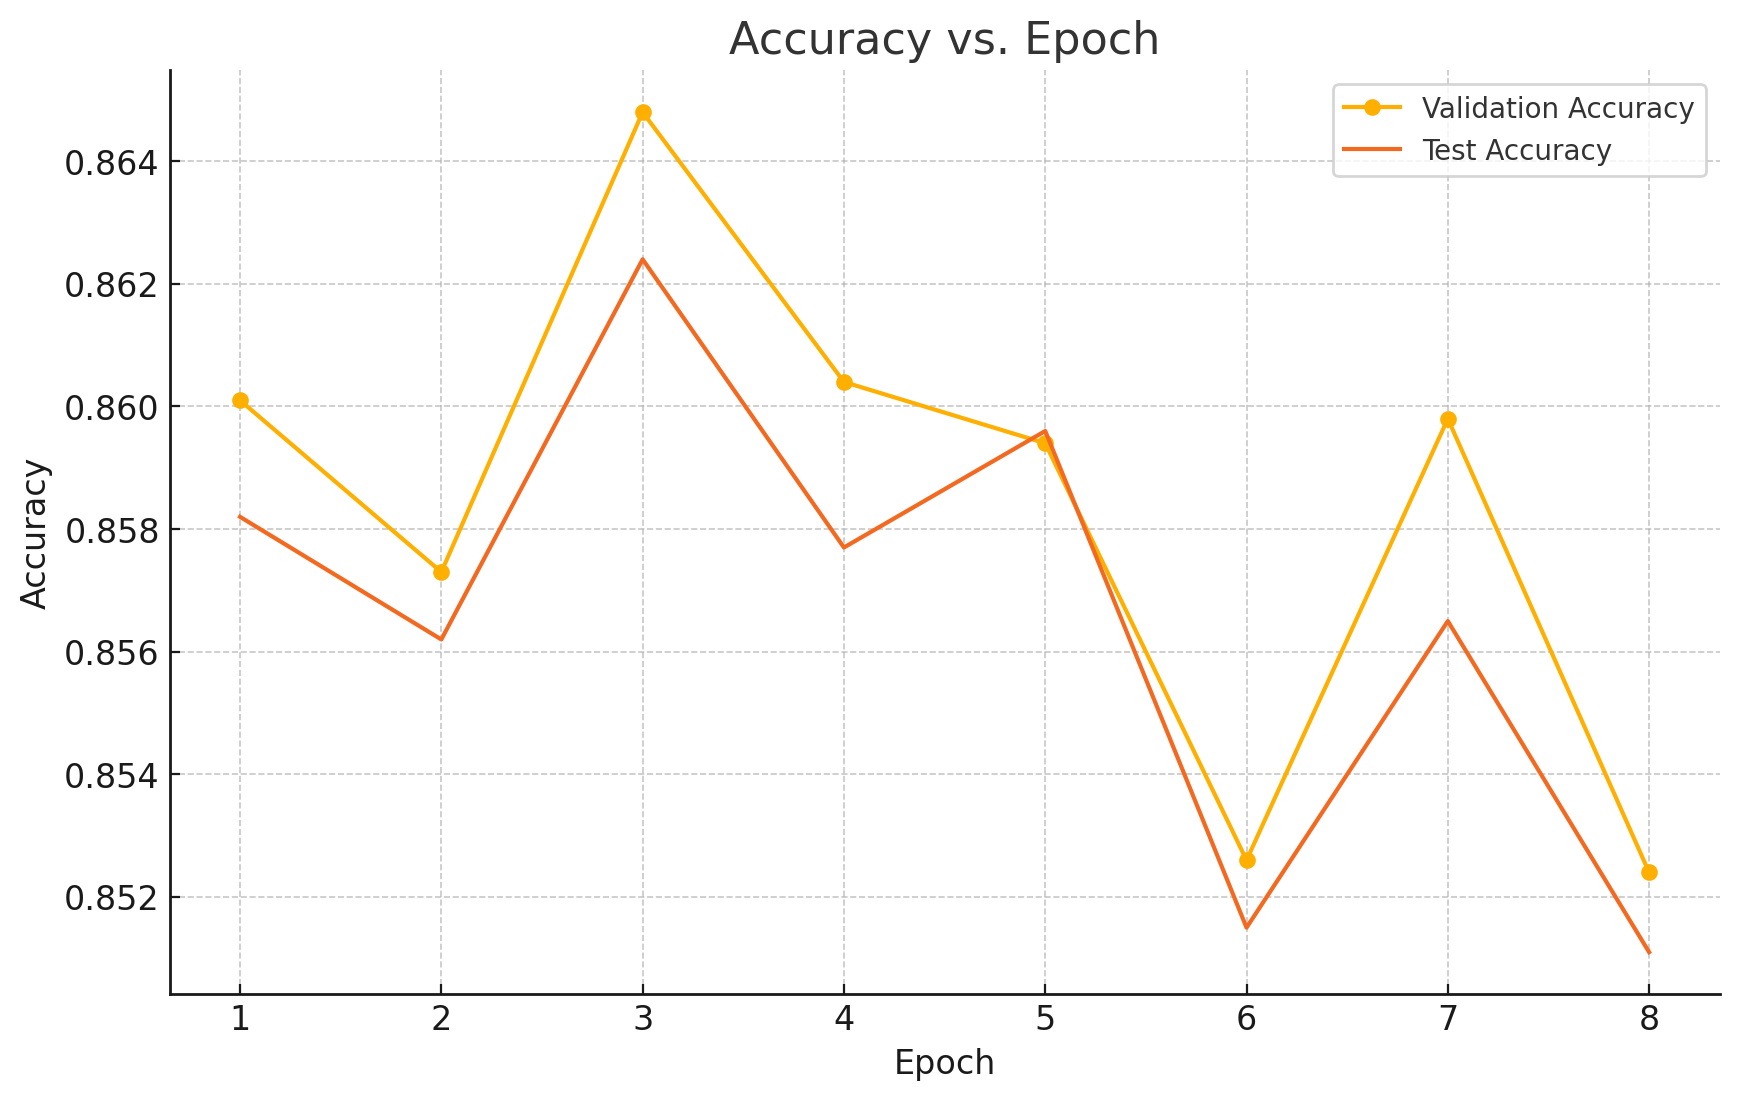
\includegraphics[width=0.5\linewidth,height=\textheight,keepaspectratio]{images/Robertector_Accuracy.png}
\caption{learning plot on accuracy}
\end{figure}

\begin{figure}
\centering
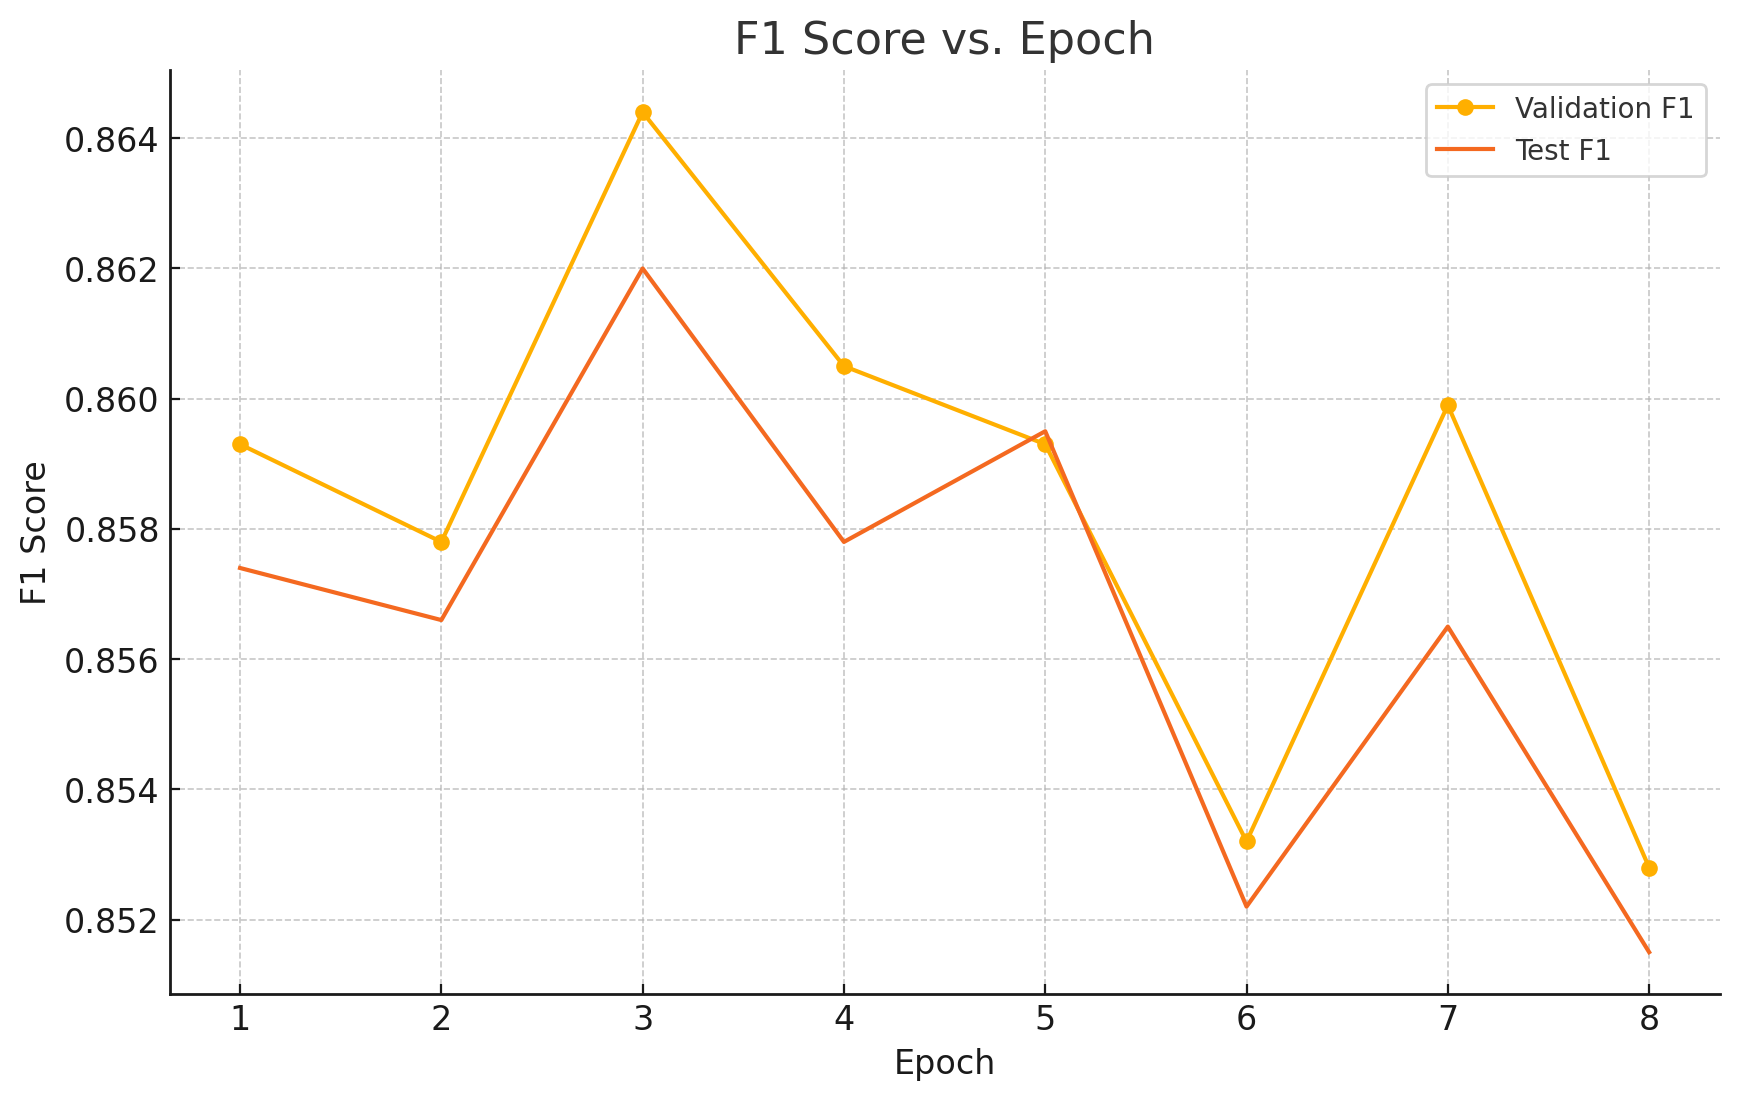
\includegraphics[width=0.5\linewidth,height=\textheight,keepaspectratio]{images/Robertector_F1.png}
\caption{learning plot on F1 score}
\end{figure}

model from epoch 3 was chosen.

\subsection{Training Multi Attention
layer}\label{training-multi-attention-layer-1}

\begin{figure}
\centering
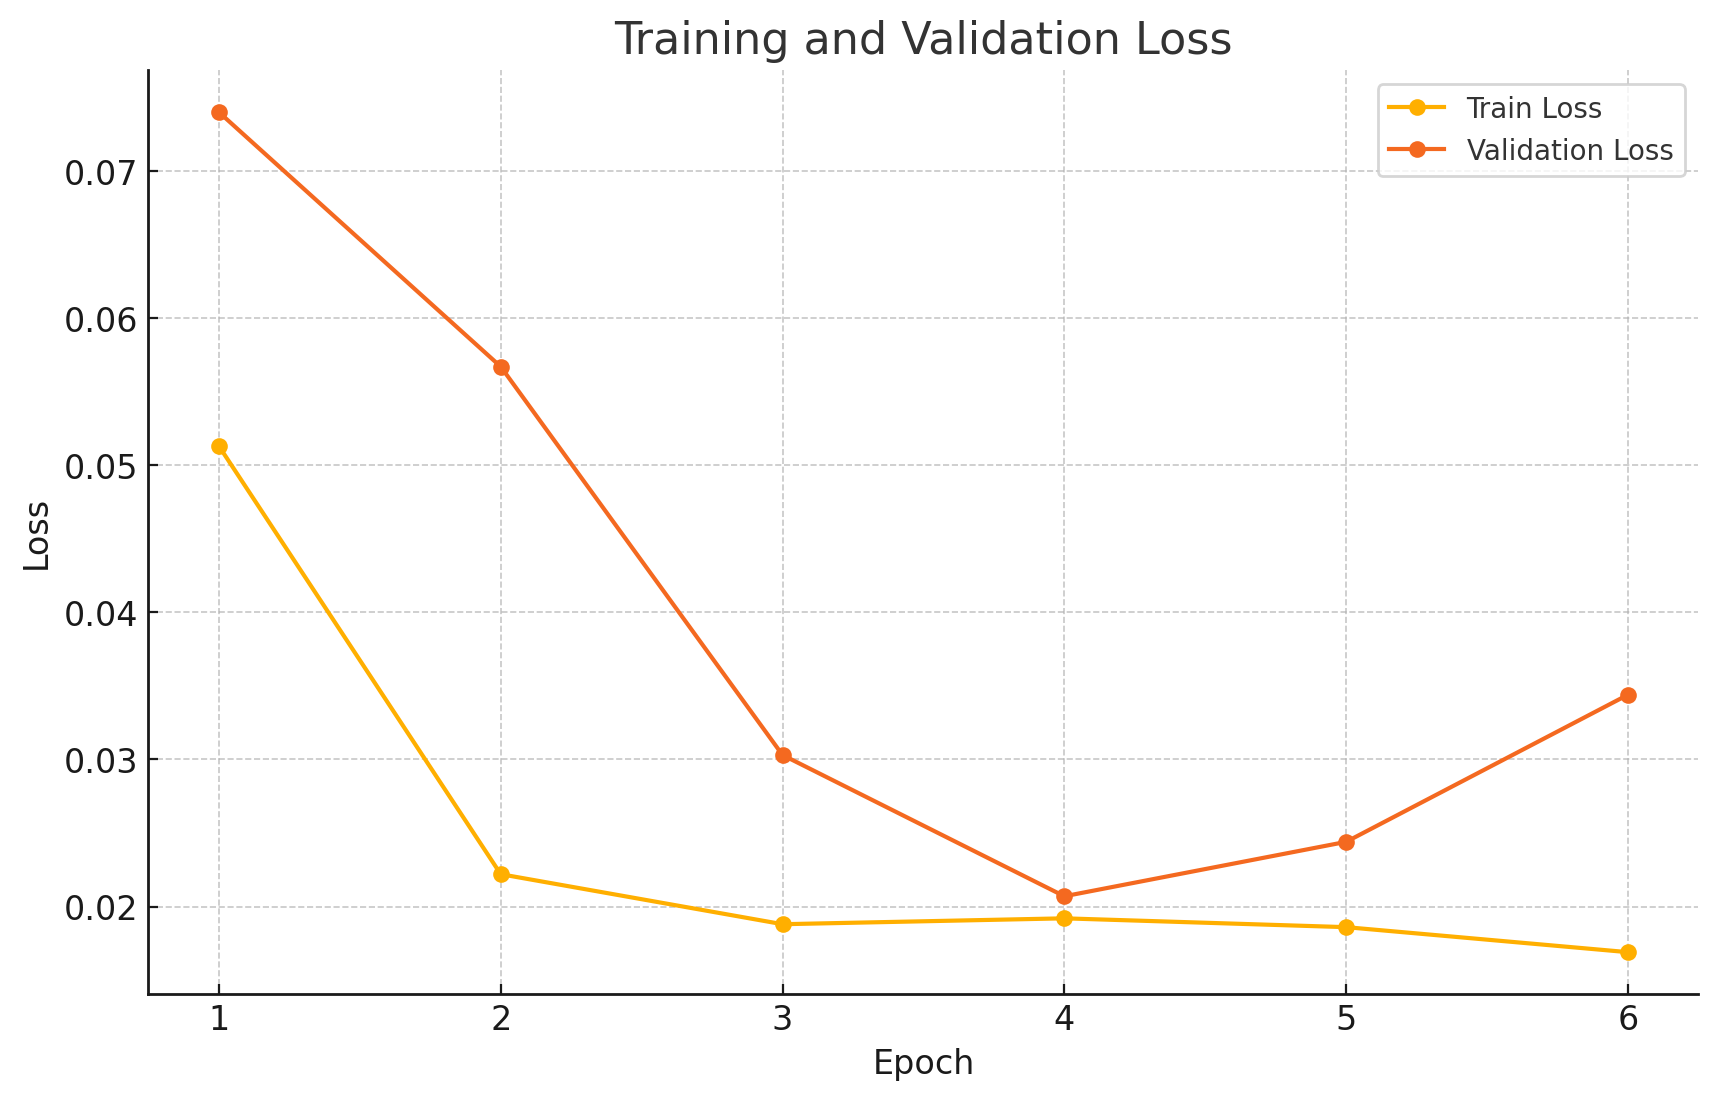
\includegraphics[width=0.5\linewidth,height=\textheight,keepaspectratio]{images/learning_plot_loss.png}
\caption{learning plot}
\end{figure}

\begin{figure}
\centering
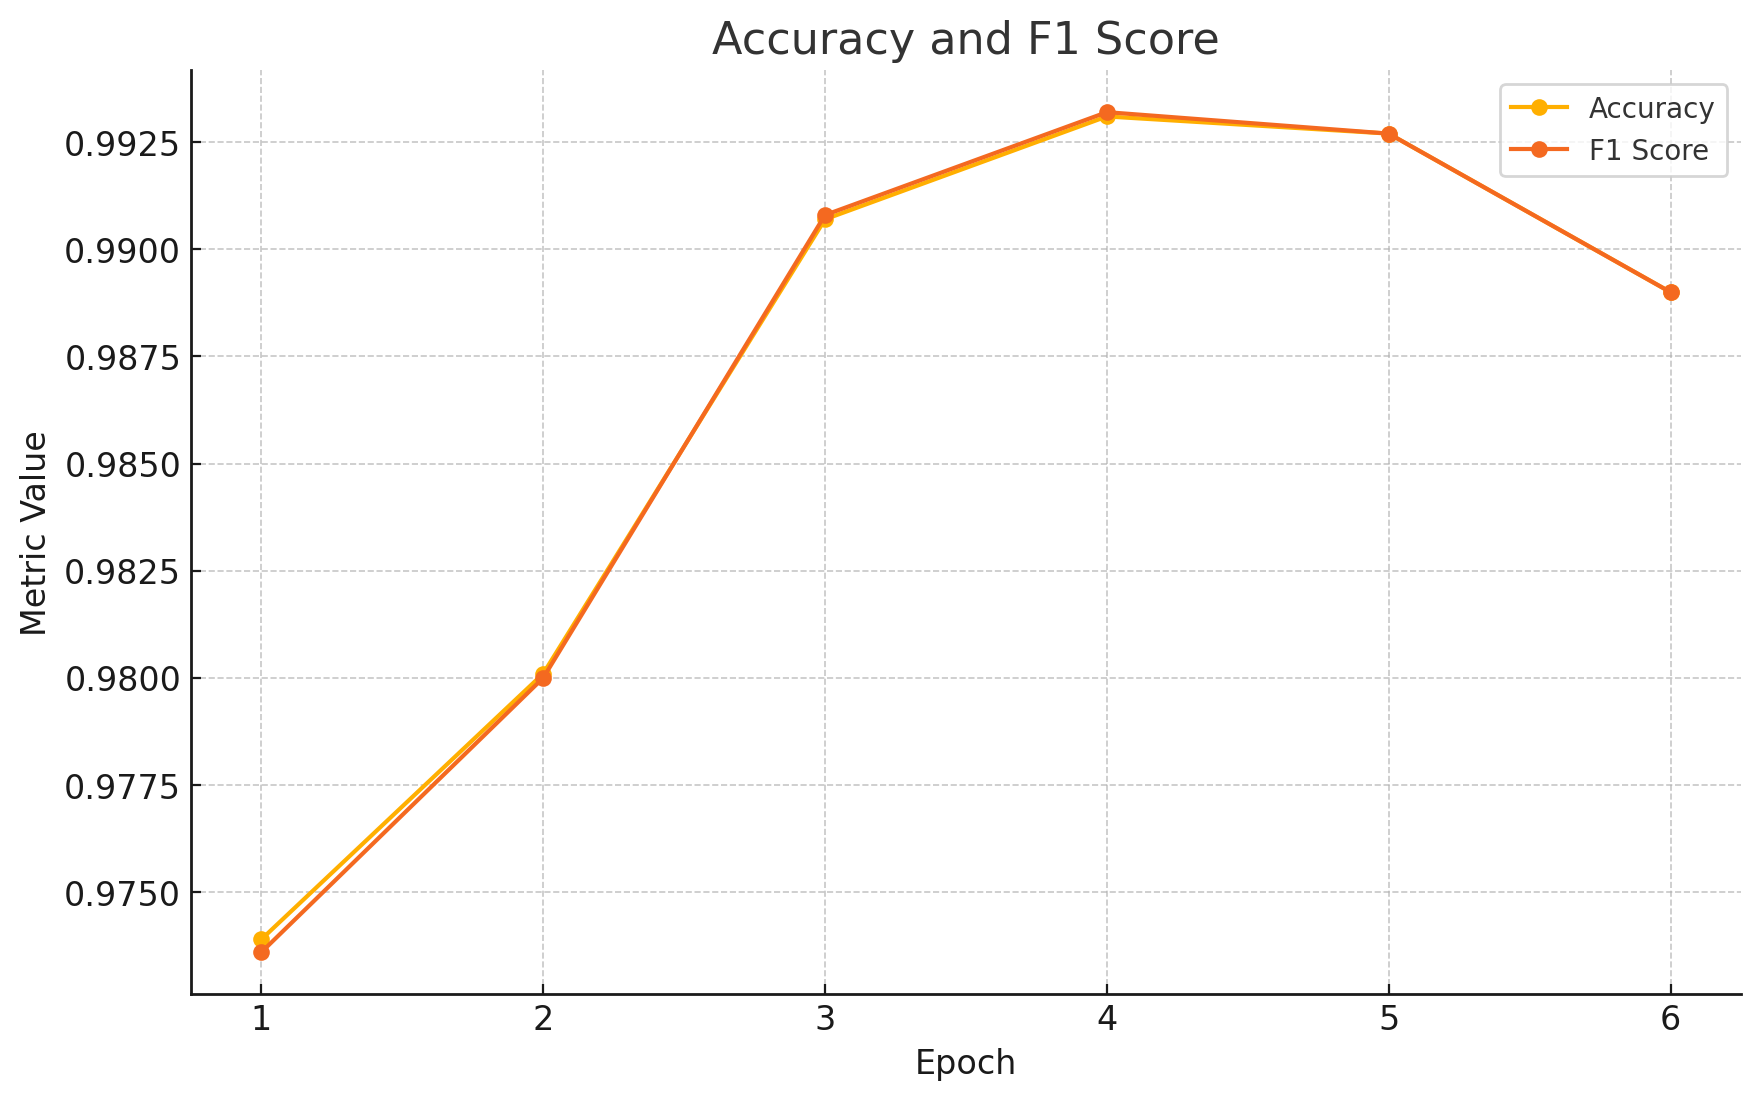
\includegraphics[width=0.5\linewidth,height=\textheight,keepaspectratio]{images/learning_plot_scores.png}
\caption{Accurracy over epochs}
\end{figure}

model from epoch 4 was chosen.

\section{\textless\textless\textless\textless\textless\textless\textless{}
Updated upstream}\label{updated-upstream}

\subsection{Graph Drawing Using R}\label{graph-drawing-using-r}

\begin{quote}
\begin{quote}
\begin{quote}
\begin{quote}
\begin{quote}
\begin{quote}
\begin{quote}
Stashed changes \#\#\# Weekly Proportion and its Smooth Line
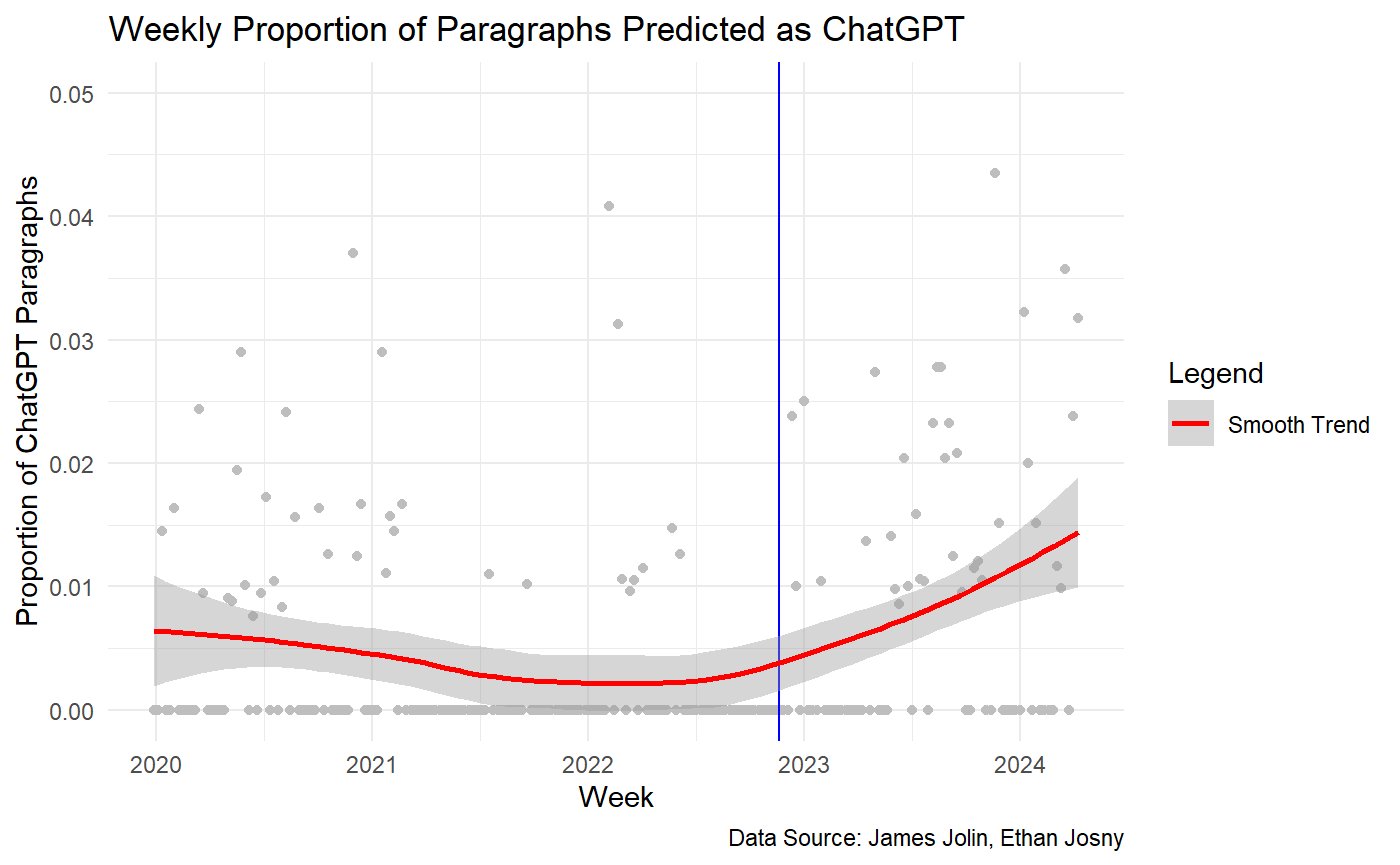
\includegraphics[width=0.5\linewidth,height=\textheight,keepaspectratio]{images/weekly_smooth.png}
\end{quote}
\end{quote}
\end{quote}
\end{quote}
\end{quote}
\end{quote}
\end{quote}

This graph shows

\begin{Shaded}
\begin{Highlighting}[]
\FunctionTok{library}\NormalTok{(tidyverse)}
\FunctionTok{library}\NormalTok{(lubridate)}

\CommentTok{\# Load and Preprocess Data}
\NormalTok{df }\OtherTok{\textless{}{-}} \FunctionTok{read\_csv}\NormalTok{(}\StringTok{"data/prob.csv"}\NormalTok{)}

\CommentTok{\# Invert Probabilities (AI = 1, Human = 0)}
\NormalTok{df }\OtherTok{\textless{}{-}}\NormalTok{ df }\SpecialCharTok{\%\textgreater{}\%}
  \FunctionTok{mutate}\NormalTok{(}\AttributeTok{probability =} \DecValTok{1} \SpecialCharTok{{-}}\NormalTok{ probability,}
         \AttributeTok{prediction =} \DecValTok{1} \SpecialCharTok{{-}}\NormalTok{ prediction,}
         \AttributeTok{Week =} \FunctionTok{floor\_date}\NormalTok{(}\FunctionTok{as.Date}\NormalTok{(Date), }\AttributeTok{unit =} \StringTok{"week"}\NormalTok{))}

\CommentTok{\# Weekly Mean Calculation}
\NormalTok{df\_mean }\OtherTok{\textless{}{-}}\NormalTok{ df }\SpecialCharTok{\%\textgreater{}\%}
  \FunctionTok{group\_by}\NormalTok{(Week) }\SpecialCharTok{\%\textgreater{}\%}
  \FunctionTok{summarise}\NormalTok{(}\AttributeTok{mean\_chatgpt =} \FunctionTok{mean}\NormalTok{(prediction), }\AttributeTok{.groups =} \StringTok{"drop"}\NormalTok{)}

\CommentTok{\# GPT Release Date}
\NormalTok{gpt\_date }\OtherTok{\textless{}{-}} \FunctionTok{floor\_date}\NormalTok{(}\FunctionTok{as.Date}\NormalTok{(}\StringTok{"2022{-}11{-}21"}\NormalTok{), }\AttributeTok{unit =} \StringTok{"week"}\NormalTok{)}

\CommentTok{\# Subsets for Pre and Post{-}GPT}
\NormalTok{df\_pre\_gpt }\OtherTok{\textless{}{-}}\NormalTok{ df }\SpecialCharTok{\%\textgreater{}\%} \FunctionTok{filter}\NormalTok{(Week }\SpecialCharTok{\textless{}=}\NormalTok{ gpt\_date)}
\NormalTok{df\_post\_gpt }\OtherTok{\textless{}{-}}\NormalTok{ df }\SpecialCharTok{\%\textgreater{}\%} \FunctionTok{filter}\NormalTok{(Week }\SpecialCharTok{\textgreater{}}\NormalTok{ gpt\_date)}

\CommentTok{\# Plot 1: Smoothed Trend Line with Points}
\FunctionTok{ggplot}\NormalTok{(}\AttributeTok{data =}\NormalTok{ df\_mean, }\FunctionTok{aes}\NormalTok{(}\AttributeTok{x =}\NormalTok{ Week, }\AttributeTok{y =}\NormalTok{ mean\_chatgpt)) }\SpecialCharTok{+}
  \FunctionTok{geom\_point}\NormalTok{(}\AttributeTok{color =} \StringTok{"gray"}\NormalTok{) }\SpecialCharTok{+}
  \FunctionTok{geom\_vline}\NormalTok{(}\AttributeTok{xintercept =}\NormalTok{ gpt\_date, }\AttributeTok{color =} \StringTok{"blue"}\NormalTok{) }\SpecialCharTok{+}
  \FunctionTok{geom\_smooth}\NormalTok{(}\FunctionTok{aes}\NormalTok{(}\AttributeTok{color =} \StringTok{"Smooth Trend"}\NormalTok{), }\AttributeTok{se =} \ConstantTok{TRUE}\NormalTok{) }\SpecialCharTok{+}
  \FunctionTok{scale\_color\_manual}\NormalTok{(}\AttributeTok{values =} \FunctionTok{c}\NormalTok{(}\StringTok{"Smooth Trend"} \OtherTok{=} \StringTok{"red"}\NormalTok{)) }\SpecialCharTok{+}
  \FunctionTok{coord\_cartesian}\NormalTok{(}\AttributeTok{ylim =} \FunctionTok{c}\NormalTok{(}\DecValTok{0}\NormalTok{, }\FloatTok{0.05}\NormalTok{)) }\SpecialCharTok{+}
  \FunctionTok{theme\_minimal}\NormalTok{() }\SpecialCharTok{+}
  \FunctionTok{labs}\NormalTok{(}\AttributeTok{x =} \StringTok{"Week"}\NormalTok{,}
       \AttributeTok{y =} \StringTok{"Proportion of ChatGPT Paragraphs"}\NormalTok{,}
       \AttributeTok{title =} \StringTok{"Weekly Proportion of Paragraphs Predicted as ChatGPT"}\NormalTok{,}
       \AttributeTok{caption =} \StringTok{"Data Source: James Jolin, Ethan Josny"}\NormalTok{,}
       \AttributeTok{color =} \StringTok{"Legend"}\NormalTok{)}
\end{Highlighting}
\end{Shaded}

\pandocbounded{\includegraphics[keepaspectratio]{Final-project_files/figure-latex/unnamed-chunk-8-1.pdf}}

\subsubsection{Average of Pre-GPT,
Post\_GPT}\label{average-of-pre-gpt-post_gpt}

\begin{figure}
\centering
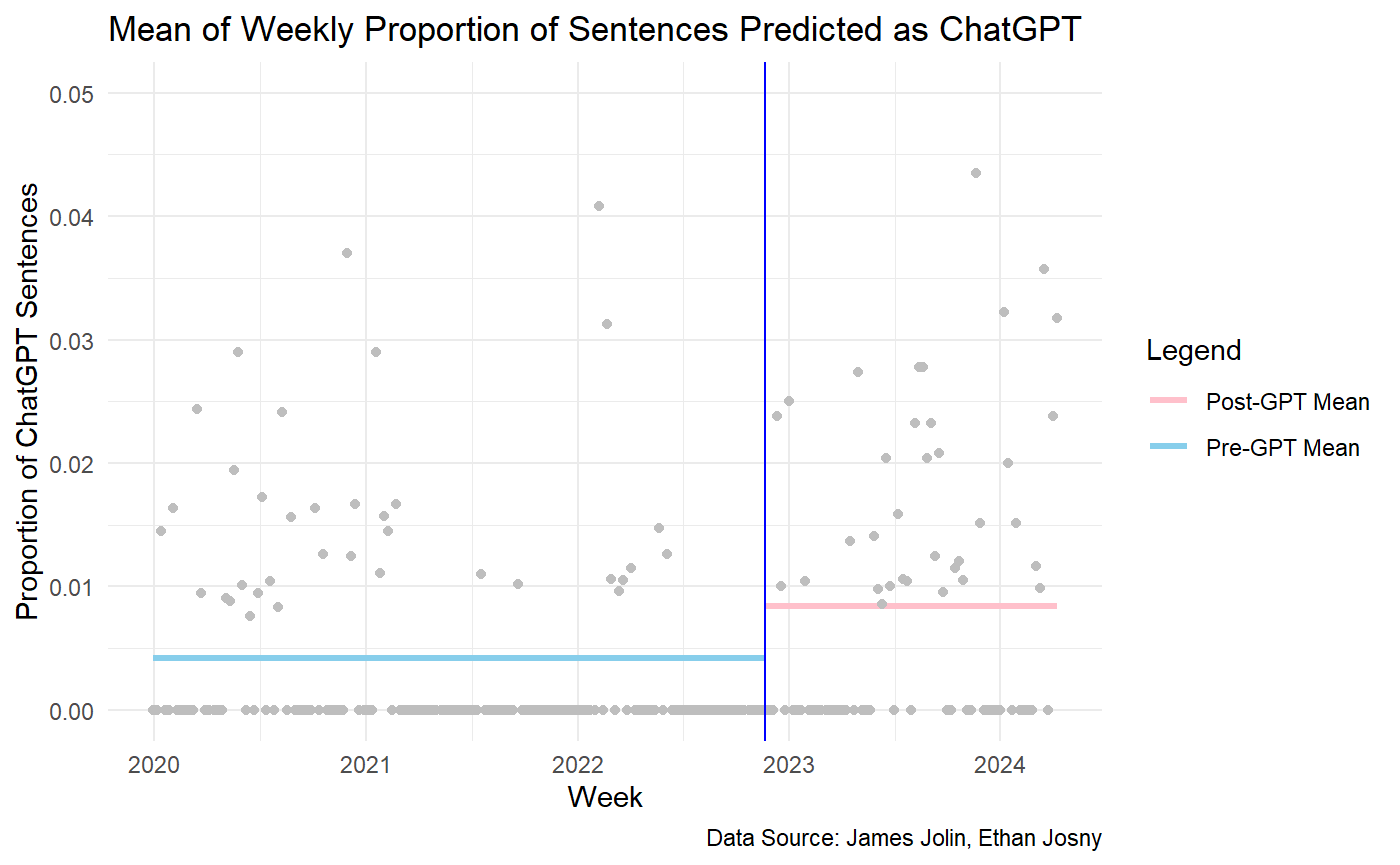
\includegraphics[width=0.5\linewidth,height=\textheight,keepaspectratio]{images/weekly_mean.png}
\caption{Mean of pre-GPT and post-GPT weekly proportion}
\end{figure}

\begin{Shaded}
\begin{Highlighting}[]
\CommentTok{\# Calculate Pre/Post GPT Means}
\NormalTok{pre\_mean }\OtherTok{\textless{}{-}} \FunctionTok{mean}\NormalTok{(df\_pre\_gpt}\SpecialCharTok{$}\NormalTok{prediction)}
\NormalTok{post\_mean }\OtherTok{\textless{}{-}} \FunctionTok{mean}\NormalTok{(df\_post\_gpt}\SpecialCharTok{$}\NormalTok{prediction)}

\CommentTok{\# Plot 2: Pre/Post GPT Mean Lines}
\FunctionTok{ggplot}\NormalTok{(}\AttributeTok{data =}\NormalTok{ df\_mean, }\FunctionTok{aes}\NormalTok{(}\AttributeTok{x =}\NormalTok{ Week, }\AttributeTok{y =}\NormalTok{ mean\_chatgpt)) }\SpecialCharTok{+}
  \FunctionTok{geom\_segment}\NormalTok{(}\FunctionTok{aes}\NormalTok{(}\AttributeTok{x =} \FunctionTok{min}\NormalTok{(Week), }\AttributeTok{xend =}\NormalTok{ gpt\_date,}
                   \AttributeTok{y =}\NormalTok{ pre\_mean, }\AttributeTok{yend =}\NormalTok{ pre\_mean, }\AttributeTok{color =} \StringTok{"Pre{-}GPT Mean"}\NormalTok{),}
               \AttributeTok{size =} \FloatTok{1.2}\NormalTok{) }\SpecialCharTok{+}
  \FunctionTok{geom\_segment}\NormalTok{(}\FunctionTok{aes}\NormalTok{(}\AttributeTok{x =}\NormalTok{ gpt\_date, }\AttributeTok{xend =} \FunctionTok{max}\NormalTok{(Week),}
                   \AttributeTok{y =}\NormalTok{ post\_mean, }\AttributeTok{yend =}\NormalTok{ post\_mean, }\AttributeTok{color =} \StringTok{"Post{-}GPT Mean"}\NormalTok{),}
               \AttributeTok{size =} \FloatTok{1.2}\NormalTok{) }\SpecialCharTok{+}
  \FunctionTok{scale\_color\_manual}\NormalTok{(}\AttributeTok{values =} \FunctionTok{c}\NormalTok{(}\StringTok{"Pre{-}GPT Mean"} \OtherTok{=} \StringTok{"skyblue"}\NormalTok{, }\StringTok{"Post{-}GPT Mean"} \OtherTok{=} \StringTok{"pink"}\NormalTok{)) }\SpecialCharTok{+}
  \FunctionTok{geom\_point}\NormalTok{(}\AttributeTok{color =} \StringTok{"gray"}\NormalTok{) }\SpecialCharTok{+}
  \FunctionTok{geom\_vline}\NormalTok{(}\AttributeTok{xintercept =}\NormalTok{ gpt\_date, }\AttributeTok{color =} \StringTok{"blue"}\NormalTok{) }\SpecialCharTok{+}
  \FunctionTok{coord\_cartesian}\NormalTok{(}\AttributeTok{ylim =} \FunctionTok{c}\NormalTok{(}\DecValTok{0}\NormalTok{, }\FloatTok{0.05}\NormalTok{)) }\SpecialCharTok{+}
  \FunctionTok{theme\_minimal}\NormalTok{() }\SpecialCharTok{+}
  \FunctionTok{labs}\NormalTok{(}\AttributeTok{x =} \StringTok{"Week"}\NormalTok{,}
       \AttributeTok{y =} \StringTok{"Proportion of ChatGPT Sentences"}\NormalTok{,}
       \AttributeTok{title =} \StringTok{"Mean of Weekly Proportion of Sentences Predicted as ChatGPT"}\NormalTok{,}
       \AttributeTok{caption =} \StringTok{"Data Source: James Jolin, Ethan Josny"}\NormalTok{,}
       \AttributeTok{color =} \StringTok{"Legend"}\NormalTok{)}
\end{Highlighting}
\end{Shaded}

\pandocbounded{\includegraphics[keepaspectratio]{Final-project_files/figure-latex/unnamed-chunk-9-1.pdf}}

\subsubsection{Linear Regression of
Post-GPT}\label{linear-regression-of-post-gpt}

\begin{figure}
\centering
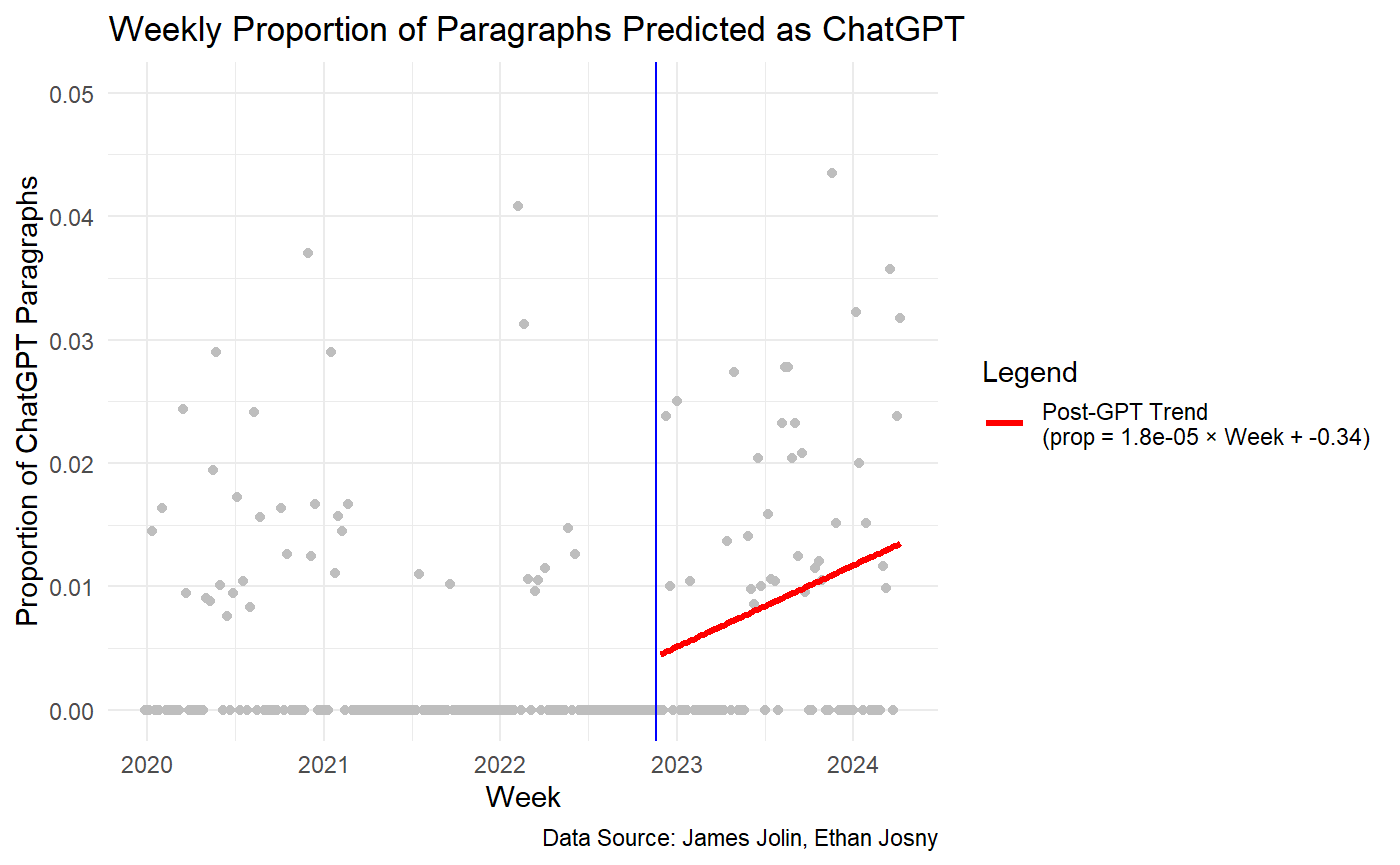
\includegraphics[width=0.5\linewidth,height=\textheight,keepaspectratio]{images/weekly_lm.png}
\caption{Weekly proportion and post-GPT linear regression model}
\end{figure}

\begin{Shaded}
\begin{Highlighting}[]
\CommentTok{\# Dataframe Storing Post GPT\textquotesingle{}s ChatGPT Proportion}
\NormalTok{df\_post\_mean }\OtherTok{\textless{}{-}}\NormalTok{ df\_mean }\SpecialCharTok{\%\textgreater{}\%} \FunctionTok{filter}\NormalTok{(Week }\SpecialCharTok{\textgreater{}}\NormalTok{ gpt\_date)}

\CommentTok{\# Linear Regression Model}
\NormalTok{model }\OtherTok{\textless{}{-}} \FunctionTok{lm}\NormalTok{(mean\_chatgpt }\SpecialCharTok{\textasciitilde{}}\NormalTok{ Week, }\AttributeTok{data =}\NormalTok{ df\_post\_mean)}
\NormalTok{co }\OtherTok{\textless{}{-}} \FunctionTok{coef}\NormalTok{(model)}

\CommentTok{\# Stores Linear Regression\textquotesingle{}s Estimation Result}
\NormalTok{df\_post\_mean }\OtherTok{\textless{}{-}} \FunctionTok{cbind}\NormalTok{(df\_post\_mean, }\FunctionTok{predict}\NormalTok{(model, }\AttributeTok{interval =} \StringTok{\textquotesingle{}confidence\textquotesingle{}}\NormalTok{))}

\CommentTok{\# Get\textquotesingle{}s Linear Model\textquotesingle{}s Equation}
\NormalTok{equation }\OtherTok{\textless{}{-}} \FunctionTok{paste}\NormalTok{(}\StringTok{"prop ="}\NormalTok{, }\FunctionTok{round}\NormalTok{(co[}\DecValTok{2}\NormalTok{], }\DecValTok{6}\NormalTok{), }\StringTok{"× Week +"}\NormalTok{, }\FunctionTok{round}\NormalTok{(co[}\DecValTok{1}\NormalTok{], }\DecValTok{2}\NormalTok{))}
\NormalTok{legend\_label }\OtherTok{\textless{}{-}} \FunctionTok{paste}\NormalTok{(}\StringTok{"Post{-}GPT Trend}\SpecialCharTok{\textbackslash{}n}\StringTok{("}\NormalTok{, equation, }\StringTok{")"}\NormalTok{, }\AttributeTok{sep =} \StringTok{""}\NormalTok{)}
\NormalTok{df\_post\_mean}\SpecialCharTok{$}\NormalTok{legend }\OtherTok{\textless{}{-}}\NormalTok{ legend\_label}

\CommentTok{\# Plot 3: Linear Regression After GPT Release}
\FunctionTok{ggplot}\NormalTok{(}\AttributeTok{data =}\NormalTok{ df\_mean, }\FunctionTok{aes}\NormalTok{(}\AttributeTok{x =}\NormalTok{ Week, }\AttributeTok{y =}\NormalTok{ mean\_chatgpt)) }\SpecialCharTok{+}
  \FunctionTok{geom\_point}\NormalTok{(}\AttributeTok{color =} \StringTok{"gray"}\NormalTok{) }\SpecialCharTok{+}
  \FunctionTok{geom\_vline}\NormalTok{(}\AttributeTok{xintercept =}\NormalTok{ gpt\_date, }\AttributeTok{color =} \StringTok{"blue"}\NormalTok{) }\SpecialCharTok{+}
  \FunctionTok{geom\_line}\NormalTok{(}\AttributeTok{data =}\NormalTok{ df\_post\_mean, }\FunctionTok{aes}\NormalTok{(}\AttributeTok{x =}\NormalTok{ Week, }\AttributeTok{y =}\NormalTok{ fit, }\AttributeTok{color =}\NormalTok{ legend), }\AttributeTok{size =} \FloatTok{1.2}\NormalTok{) }\SpecialCharTok{+}
  \FunctionTok{scale\_color\_manual}\NormalTok{(}\AttributeTok{values =} \FunctionTok{setNames}\NormalTok{(}\StringTok{"red"}\NormalTok{, legend\_label)) }\SpecialCharTok{+}
  \FunctionTok{coord\_cartesian}\NormalTok{(}\AttributeTok{ylim =} \FunctionTok{c}\NormalTok{(}\DecValTok{0}\NormalTok{, }\FloatTok{0.05}\NormalTok{)) }\SpecialCharTok{+}
  \FunctionTok{theme\_minimal}\NormalTok{() }\SpecialCharTok{+}
  \FunctionTok{labs}\NormalTok{(}\AttributeTok{x =} \StringTok{"Week"}\NormalTok{,}
       \AttributeTok{y =} \StringTok{"Proportion of ChatGPT Paragraphs"}\NormalTok{,}
       \AttributeTok{title =} \StringTok{"Weekly Proportion of Paragraphs Predicted as ChatGPT"}\NormalTok{,}
       \AttributeTok{caption =} \StringTok{"Data Source: James Jolin, Ethan Josny"}\NormalTok{,}
       \AttributeTok{color =} \StringTok{"Legend"}\NormalTok{)}
\end{Highlighting}
\end{Shaded}

\pandocbounded{\includegraphics[keepaspectratio]{Final-project_files/figure-latex/unnamed-chunk-10-1.pdf}}

\end{document}
